\title{分散型SNSにおけるユーザの潜在要求分析}
\author{プロジェクトマネジメントコース\\
ソフトウェア開発管理グループ\\
矢吹研究室\\
1442037\\
加藤 健弥}
\date{}
\usepackage{listings}
\begin{document}
\maketitle

%本テンプレートの余白は,卒論マニュアルで指示されたものとは違っているが,1ページあたりの文字数は40文字x40行と,卒論マニュアル通りになっている。文字間隔や行間隔を調整して,余白をマニュアル通りにすることもできるが,それでは文章が読みにくくなるため,このような対応をしている。

%\noindent
□□□□□□□□□■□□□□□□□□□■□□□□□□□□□■□□□□□□□□□■
□□□□□□□□□■□□□□□□□□□■□□□□□□□□□■□□□□□□□□□■
□□□□□□□□□■□□□□□□□□□■□□□□□□□□□■□□□□□□□□□■
□□□□□□□□□■□□□□□□□□□■□□□□□□□□□■□□□□□□□□□■
□□□□□□□□□■□□□□□□□□□■□□□□□□□□□■□□□□□□□□□■
□□□□□□□□□■□□□□□□□□□■□□□□□□□□□■□□□□□□□□□■
□□□□□□□□□■□□□□□□□□□■□□□□□□□□□■□□□□□□□□□■
□□□□□□□□□■□□□□□□□□□■□□□□□□□□□■□□□□□□□□□■
□□□□□□□□□■□□□□□□□□□■□□□□□□□□□■□□□□□□□□□■
□□□□□□□□□■□□□□□□□□□■□□□□□□□□□■□□□□□□□□□■
□□□□□□□□□■□□□□□□□□□■□□□□□□□□□■□□□□□□□□□■
□□□□□□□□□■□□□□□□□□□■□□□□□□□□□■□□□□□□□□□■
□□□□□□□□□■□□□□□□□□□■□□□□□□□□□■□□□□□□□□□■
□□□□□□□□□■□□□□□□□□□■□□□□□□□□□■□□□□□□□□□■
□□□□□□□□□■□□□□□□□□□■□□□□□□□□□■□□□□□□□□□■
□□□□□□□□□■□□□□□□□□□■□□□□□□□□□■□□□□□□□□□■
□□□□□□□□□■□□□□□□□□□■□□□□□□□□□■□□□□□□□□□■
□□□□□□□□□■□□□□□□□□□■□□□□□□□□□■□□□□□□□□□■
□□□□□□□□□■□□□□□□□□□■□□□□□□□□□■□□□□□□□□□■
□□□□□□□□□■□□□□□□□□□■□□□□□□□□□■□□□□□□□□□■
□□□□□□□□□■□□□□□□□□□■□□□□□□□□□■□□□□□□□□□■
□□□□□□□□□■□□□□□□□□□■□□□□□□□□□■□□□□□□□□□■
□□□□□□□□□■□□□□□□□□□■□□□□□□□□□■□□□□□□□□□■
□□□□□□□□□■□□□□□□□□□■□□□□□□□□□■□□□□□□□□□■
□□□□□□□□□■□□□□□□□□□■□□□□□□□□□■□□□□□□□□□■
□□□□□□□□□■□□□□□□□□□■□□□□□□□□□■□□□□□□□□□■
□□□□□□□□□■□□□□□□□□□■□□□□□□□□□■□□□□□□□□□■
□□□□□□□□□■□□□□□□□□□■□□□□□□□□□■□□□□□□□□□■
□□□□□□□□□■□□□□□□□□□■□□□□□□□□□■□□□□□□□□□■
□□□□□□□□□■□□□□□□□□□■□□□□□□□□□■□□□□□□□□□■
□□□□□□□□□■□□□□□□□□□■□□□□□□□□□■□□□□□□□□□■
□□□□□□□□□■□□□□□□□□□■□□□□□□□□□■□□□□□□□□□■
□□□□□□□□□■□□□□□□□□□■□□□□□□□□□■□□□□□□□□□■
□□□□□□□□□■□□□□□□□□□■□□□□□□□□□■□□□□□□□□□■
□□□□□□□□□■□□□□□□□□□■□□□□□□□□□■□□□□□□□□□■
□□□□□□□□□■□□□□□□□□□■□□□□□□□□□■□□□□□□□□□■
□□□□□□□□□■□□□□□□□□□■□□□□□□□□□■□□□□□□□□□■
□□□□□□□□□■□□□□□□□□□■□□□□□□□□□■□□□□□□□□□■
□□□□□□□□□■□□□□□□□□□■□□□□□□□□□■□□□□□□□□□■
■■■■■■■■■■■■■■■■■■■■■■■■■■■■■■■■■■■■■■■■
□□□□□□□□□■□□□□□□□□□■□□□□□□□□□■□□□□□□□□□■%文字数チェック用

\tableofcontents%目次

\chapter{序論}
本研究では,分散型SNSと中央集権型SNSを定量的に調査,分析を行う.分散型SNSは中央集権型SNSと求められていることに違いがあるのかを調査することとした.
\chapter{背景}
スマートフォンなどの普及により,手軽にインターネットへの接続が可能になった.そのため,TwitterやFacebookなどの様々なSNS(ソーシャルネットワークサービス)が注目されるようになった.近年ではMastodonという新たなSNSの利用者が増えてきている.

Mastodonとは2016年に公開されたオープンソースソフトウェアであり,誰でも自由にサーバを立てて運用できる.そのため,TwitterやFacebookのような利用者が一つのサーバにログインする中央集権型のサービスに対してMastodonの利用者は管理者も設置場所も異なるサーバにあるインスタンスにログインする分散型のサービスである\cite{mas}.

インスタンスとは,Mastodonを運用しているそれぞれのサーバのことである.そのため,利用者は別のインスタンスの利用者とはつながっていない.しかしインスタンス同士が連合という形で結びつくことができるため,別のインスタンスであっても連合であれば利用者同士でつながることができる\cite{Mastodon}.
\chapter{目的}
TwitterとMastodonで,投稿される話題に違いがあるかを,つぶやきを定量的に分析することによって調査する.
\chapter{手法}
全体のながれとしては以下のとおりである.

\begin{enumerate}
\item TwitterのAPIキー,アクセストークンを取得する.
\item MastodonのAPIキー,アクセストークンを取得する.
\item Twitter APIを使用し,Twitterから無作為に100のつぶやきを取得する.
\item Mastodon APIを使用し,Mastodonの30のインスタンスから1つのインスタンスごとに無作為に100のつぶやきを取得する.
\item TwitterとMastodonのつぶやきをWord2vecによってベクトル化する.
\item TwitterとMastodonの各インスタンス同士で主成分分析する.
\end{enumerate}
\newpage

\section{研究の対象にするMastodonのインスタンス}

研究の対象にするMastodonのインスタンスは以下のとおりである.

\begin{enumerate}
\item aidon.club
\item bicyclemstdn.jp
\item catdon.life
\item dq10.online
\item eigadon.net
\item fgochiho.vip
\item friends.nico
\item gamecreate.mstdn.cloud
\item ika.queloud.net
\item imastodon.net
\item kero.ccsakura.jp
\item kirakiratter.com
\item konkat.jp
\item kurage.cc
\item mast.moe
\item mastodon.bitbank.cc
\item mastodon.cosmicanimal.jp
\item mastodon.fishing
\item mastodon.yokohama
\item mstdn.hokkaido.jp
\item mstdn.jp
\item mstdn.osaka
\item mstdn-football.jp
\item mstdn-kanazawa.jp
\item now.kibousoft.co.jp
\item pawoo.net
\item ro-mastodon.puyo.jp
\item toot.redmine.jp
\item tuner.1242.com
\item vocalodon.net
\end{enumerate}
\newpage
\section{研究に必要な道具の準備}
\subsection{Chocolateyの導入}


\subsubsection{Chocolateyとは}
Chocolateyとはコマンドラインで操作をすることができるWindows用パッケージマネージャーである.LinuxOSのパッケージ管理コマンドのように使うことができる.

\subsubsection{Chocolateyのインストール}
以下のようにホームページからインストールする.

\begin{figure}[h]
\centering
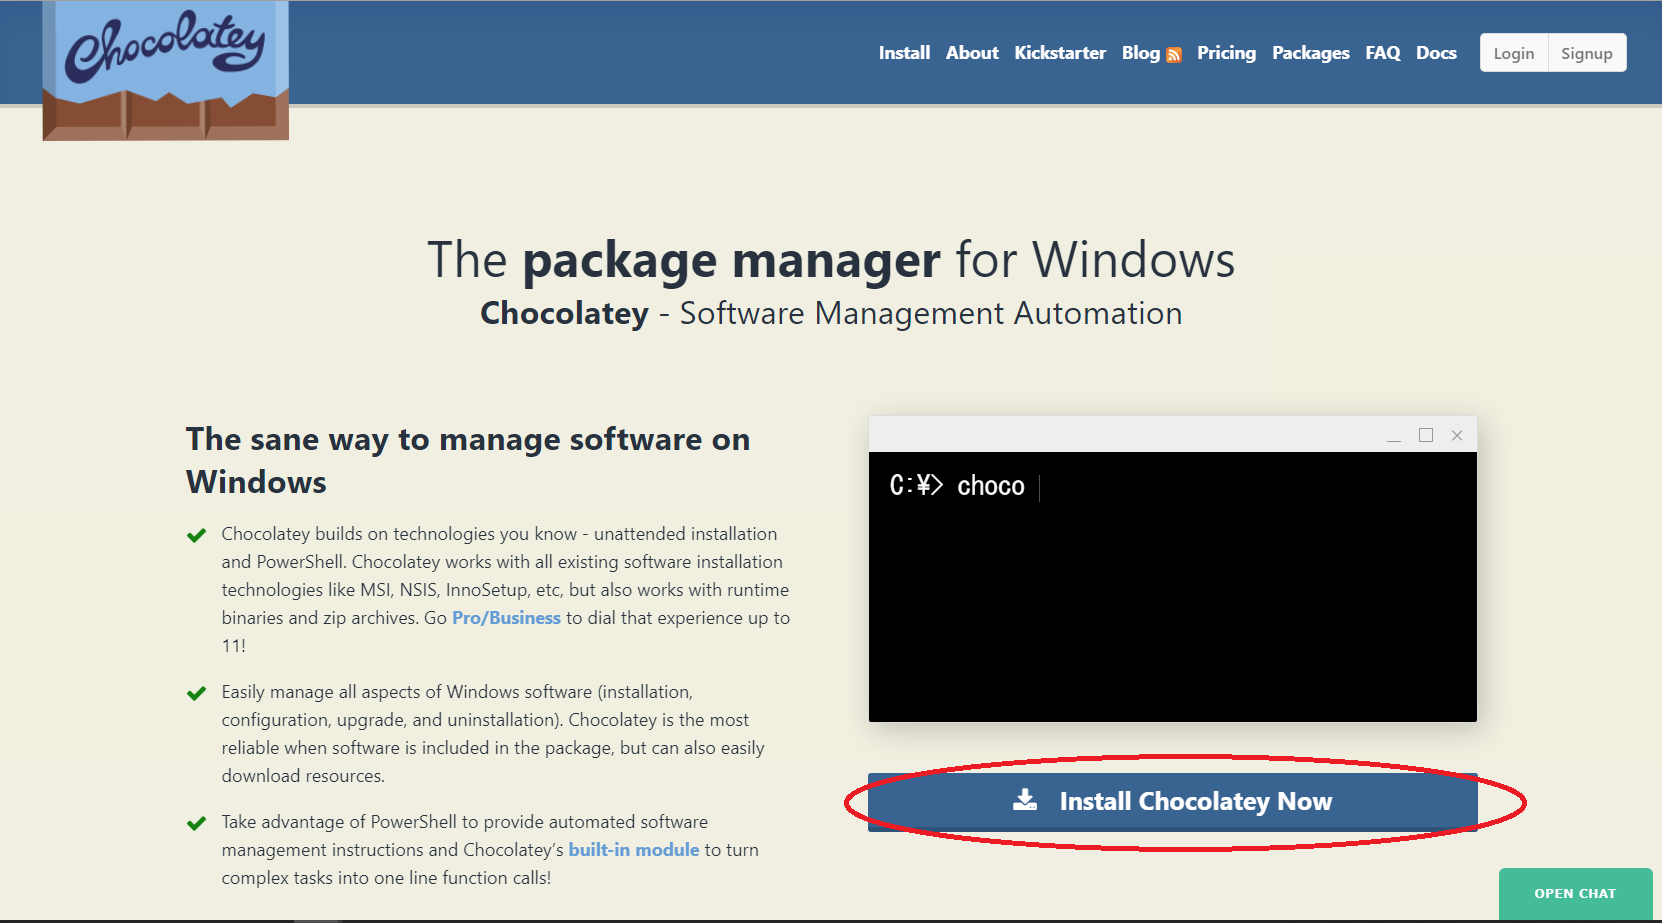
\includegraphics[width=13cm,clip]{chocolatey1.PNG}
\caption{Chocolateyのホームページ}
\end{figure}

公式ホームページのインストールページに行き,Install Chocolatey Nowを選択する.

\newpage
\begin{figure}[h]
\centering
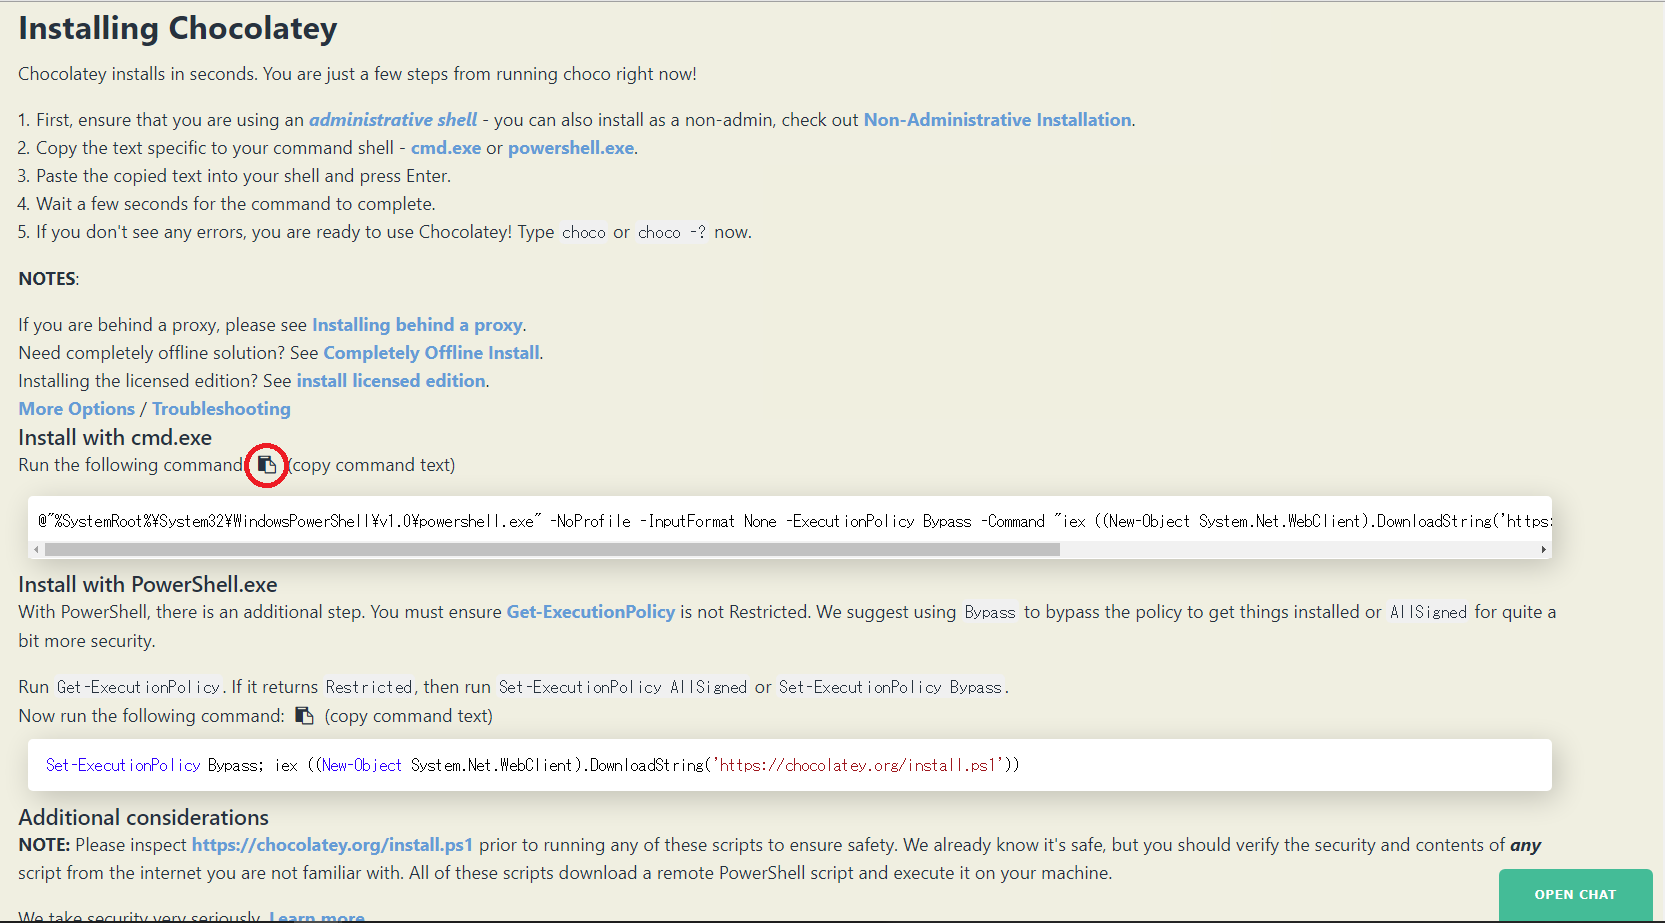
\includegraphics[width=13cm,clip]{chocolatey2.PNG}
\caption{コマンドプロンプトでインストールする場合}
\end{figure}

赤い丸の部分を選択するとコマンドプロンプトChocolateyをインストールするコマンドがコピーされる.

実際にコピーしたコマンドは以下である.

\begin{verbatim}
@"%SystemRoot%\System32\WindowsPowerShell\v1.0\powershell.exe" -NoProfile
 -InputFormat None -ExecutionPolicy Bypass -Command  "iex ((New-Object
  System.Net.WebClient).DownloadString('https://chocolatey.org/install.ps1'))" 
  && SET "PATH=%PATH%;%ALLUSERSPROFILE%\chocolatey\bin"
\end{verbatim}
\newpage
コマンドプロンプトを管理者で起動し,先ほどコピーしたコマンドを入力するとChocolateyをインストールする.以下の画面はインストールが成功画面である.

\begin{figure}[h]
\centering
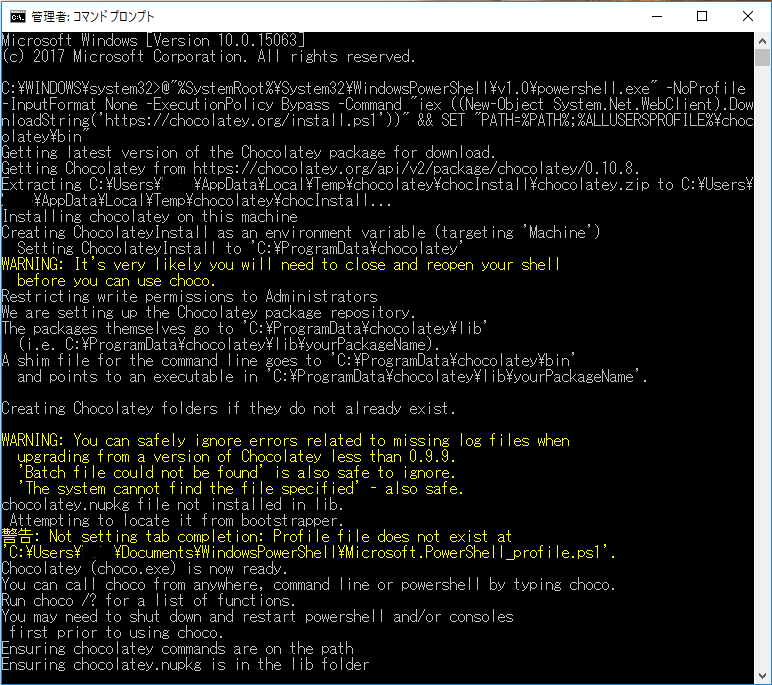
\includegraphics[width=13cm,clip]{chocolateyinst.PNG}
\caption{Chocolateyのインストール成功画面}
\end{figure}
\newpage
\subsection{Rの導入}
\subsubsection{Rとは}
Rとは統計解析ソフトであり,オープンソース・フリーソフトウェアとなっている.
\subsubsection{Chocolateyを使ったRの導入}



以下のコマンドでRをインストールする.\\

texttt{cinstl -y r.project}\\

以下の画面はインストールが成功画面である.
\begin{figure}[h]
\centering
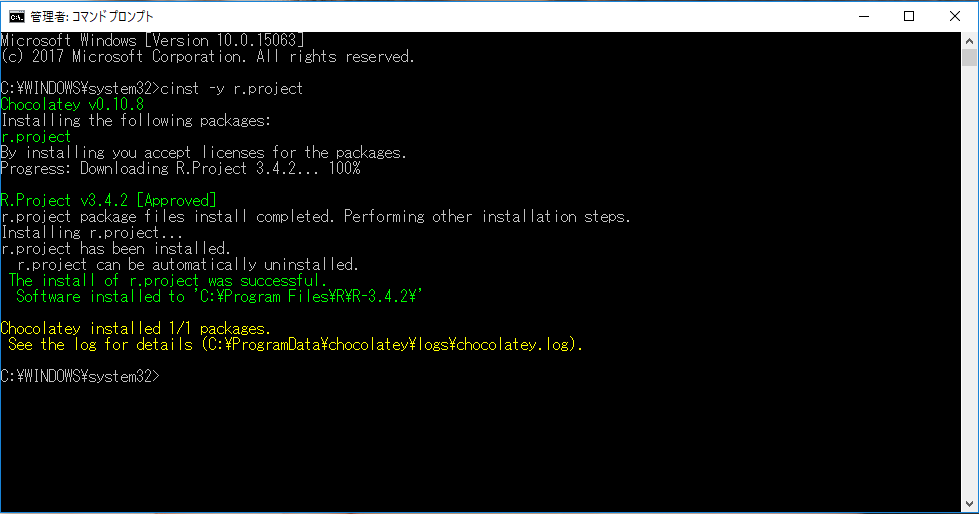
\includegraphics[width=13cm,clip]{Rinst.PNG}
\caption{Rのインストール}
\end{figure}
\newpage
\subsubsection{インストーラーを使ったRの導入}
CRAN(The Comprehensive R Archive Network)が提供するR for Windowsのインストーラーダウンロードページ(https://cran.ism.ac.jp/)にアクセスし,Download R for Windowsを選択.
\begin{figure}[h]
\centering
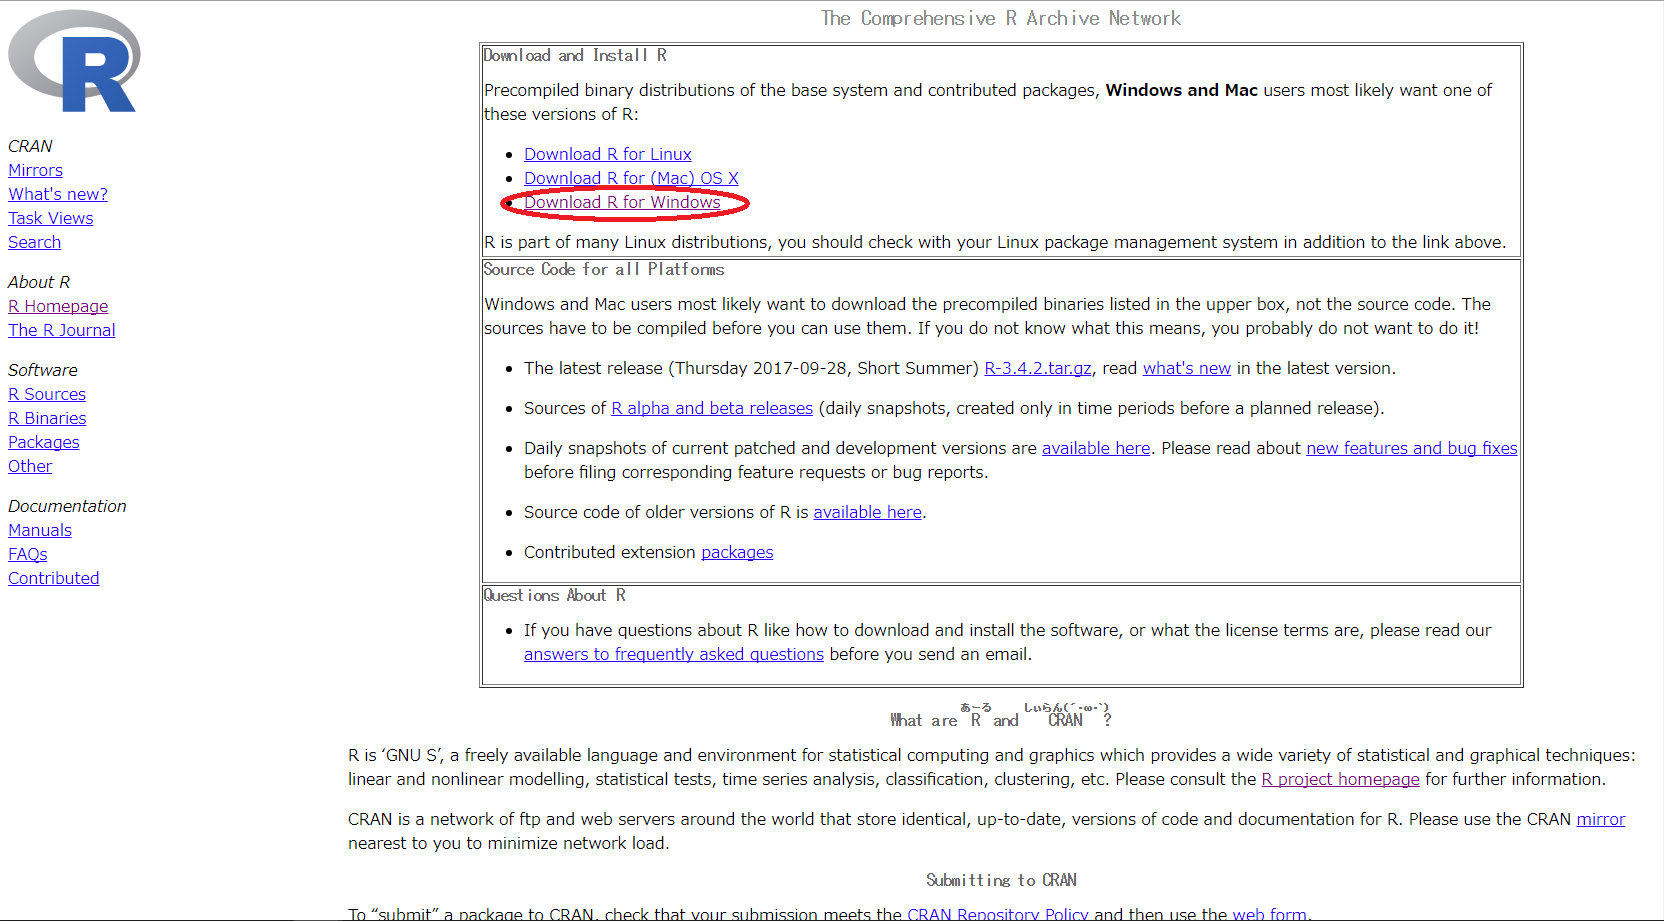
\includegraphics[width=13cm,clip]{Rdown1.PNG}
\caption{Download R for Windowsを選択}
\end{figure}
\newpage
baseをインストールするので,install R for the first timeを選択.
\begin{figure}[h]
\centering
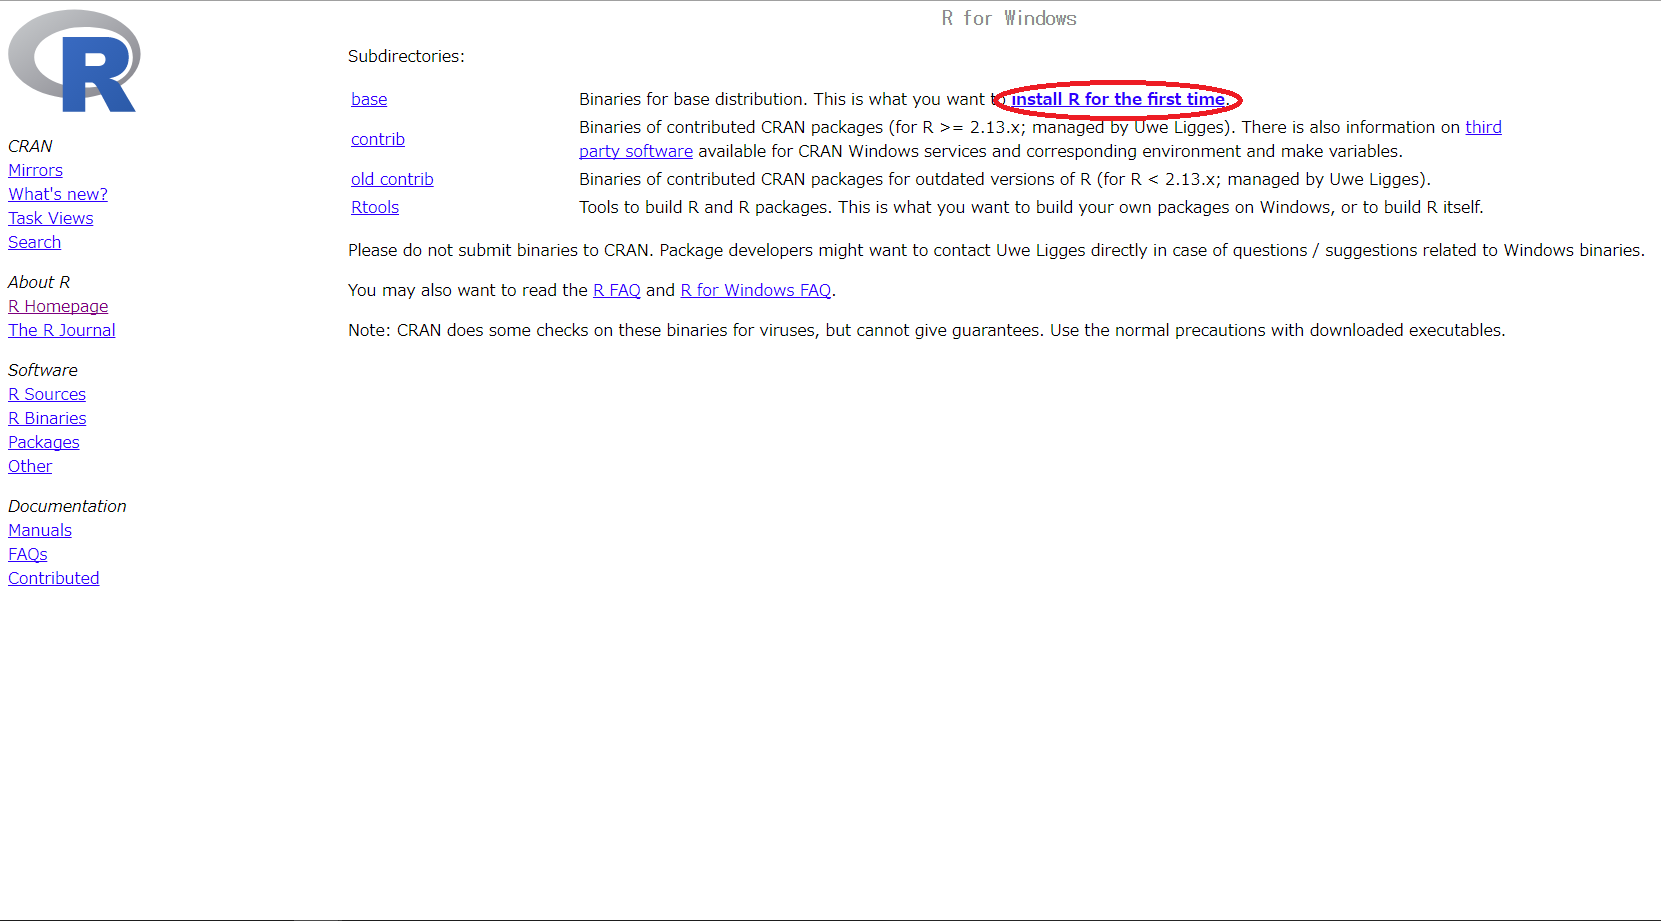
\includegraphics[width=13cm,clip]{Rdown2.PNG}
\caption{install R for the first timeを選択}
\end{figure}
\newpage
Download R 3.4.2 for Windows(3.4.2の部分はバージョンによって異なる)を選択.
\begin{figure}[h]
\centering
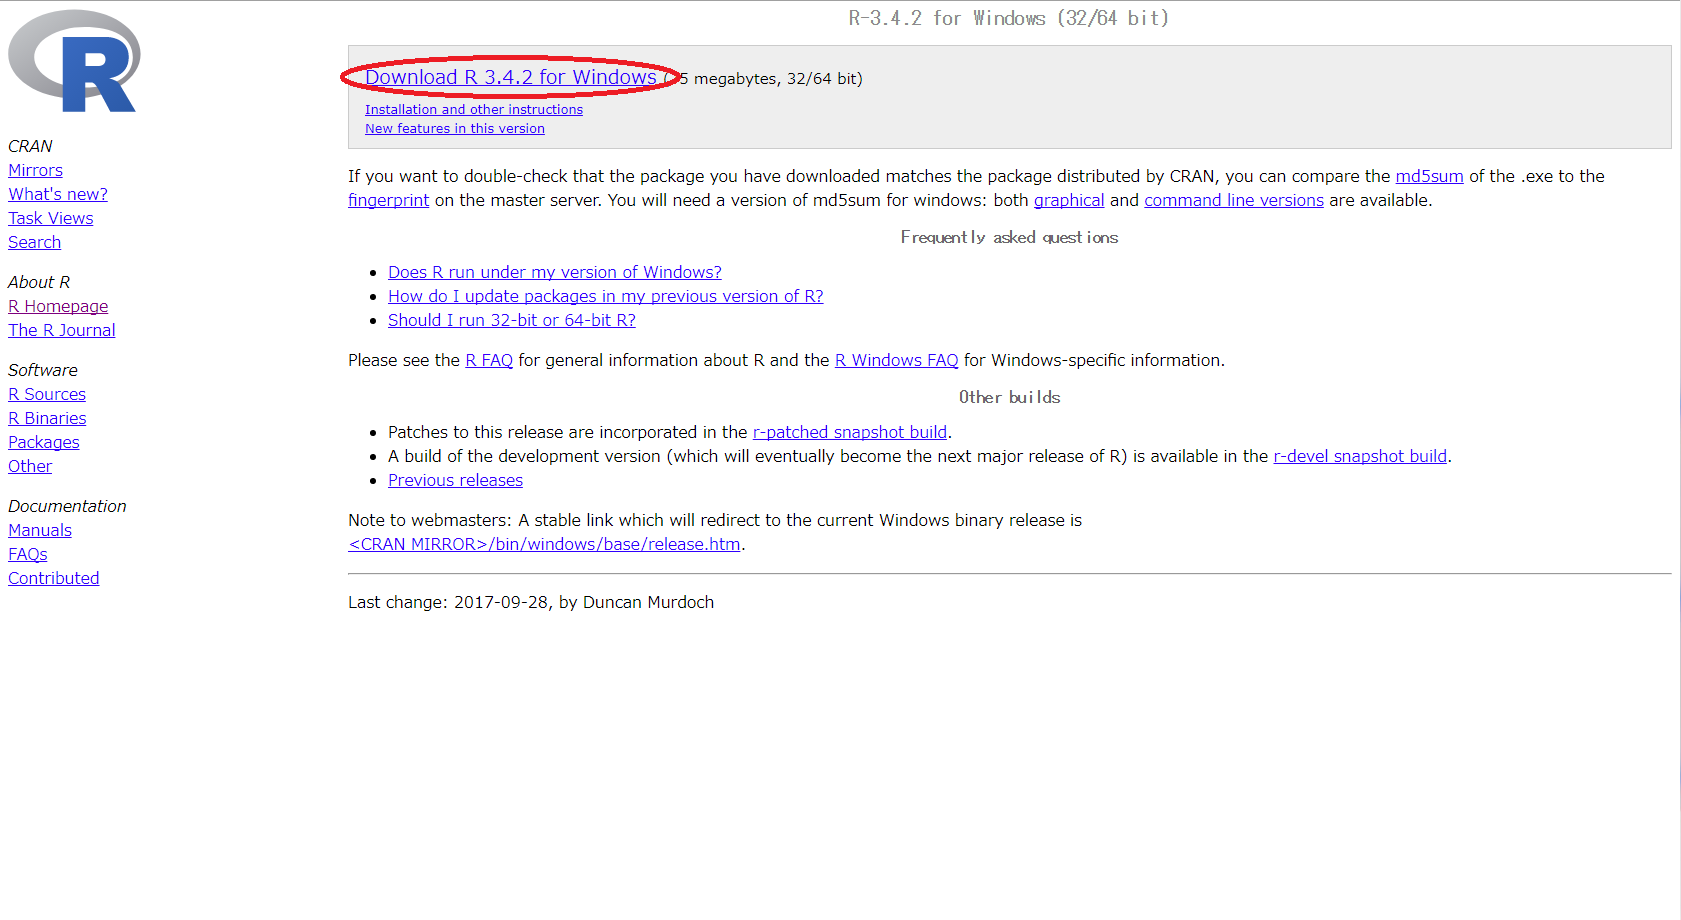
\includegraphics[width=13cm,clip]{Rdown3.PNG}
\caption{Download R 3.4.2 for Windows}
\end{figure}
\newpage

インストーラーがダウンロードできたら起動し,インストールする.

\begin{figure}[h]
\centering 
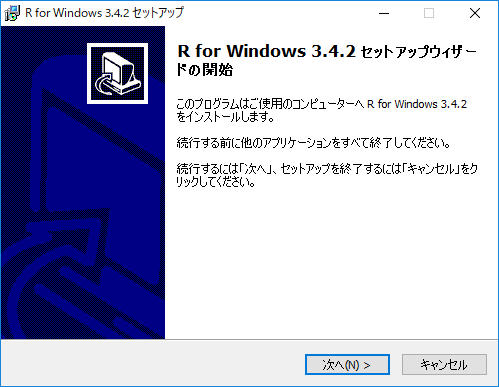
\includegraphics[width=13cm]{Rinst1.png}
\caption{Rをインストールする}
\end{figure}

\newpage
\subsection{Anacondaの導入}
\subsubsection{Anacondaとは}
PythonとPythonのライブラリをセットにしたパッケージである.
\subsubsection{Anacondaのインストール}
\begin{verbatim}
Ubuntuの起動したコマンドプロンプト内で以下のコマンドを入力する.

bash Anaconda3-5.0.1-Linux-x86_64.sh
\end{verbatim}
\subsubsection{環境変数の設定}
\begin{verbatim}
Ubuntuの起動したコマンドプロンプト内で以下のコマンドを入力する.

cat << "EOF" >> .bash_profile
export CUDA_HOME=/usr/local/cuda
export CUDA_PATH=$CUDA_HOME
export PATH=$HOME/anaconda3/bin:$CUDA_HOME/bin:$PATH
export LD_LIBRARY_PATH=$LD_LIBRARY_PATH:$CUDA_HOME/lib64:$CUDA_HOME/extras/CUPTI/lib64
EOF
\end{verbatim}
\newpage
\subsection{Twitter APIの導入}

\subsubsection{Twitter APIとは}
Twitter社が提供しているサービスで,WebサイトやアプリなどからTwitterの機能を呼び出すことができる.
このAPIを利用することでつぶやきの参照や検索などを行なえるアプリケーション開発ができるようになる.
\subsubsection{tweepyのインストール}
\begin{verbatim}
Ubuntuの起動したコマンドプロンプト内で以下のコマンドを入力する.

sudo pip install tweepy
\end{verbatim}
\subsubsection{TwitterのAPIキー,アクセストークンの取得}
(https://apps.twitter.com/)にアクセスし,で新しいアプリを作る.そこでTwitterのAPIキー,アクセストークンを取得する.Twitterのアカウントが必要なので登録しておく必要がある.登録はメールアドレスと電話番号があれば可能である.

\newpage
\subsection{Mastodon APIの導入}
\subsubsection{Mastodon APIとは}
Mastodon APIはネット上に使用方法があげられており,WebサイトやアプリなどからMastodonの機能を呼び出すことができる.
このAPIを利用することでつぶやきの参照や検索などを行なえるアプリケーション開発ができるようになる.
\subsubsection{Mastodon.pyのインストール}
\begin{verbatim}
Ubuntuの起動したコマンドプロンプト内で以下のコマンドを入力する.

sudo pip install Mastodon.py

\end{verbatim}
\subsubsection{MastodonのAPIキー,アクセストークンを取得}
以下のPythonファイルを起動することでMastodonのAPIキー,アクセストークンを取得できる.取得するためにインスタンスへ登録しておく必要がある.登録はメールアドレスがあれば可能である.
\begin{lstlisting}[breaklines = true, basicstyle=\ttfamily\footnotesize, frame=single]
from mastodon import Mastodon

Mastodon.create_app(
     'pytooterapp',
     api_base_url = '*****.jp', 
     to_file = 'Mastodon_clientcred.secret' 
)
mastodon = Mastodon(
    client_id = 'Mastodon_clientcred.secret',
    api_base_url = '*****.jp'
)
mastodon.log_in(
    'my_login_email@example.com', 
    'password', 
    to_file = 'Mastodon_usercred.secret' 
)
\end{lstlisting}
\newpage

\subsection{Word2vecの導入}
\subsubsection{MeCabのインストール}
Ubuntuの起動したコマンドプロンプト内で以下のコマンドを入力する.\\

sudo apt install -y mecab mecab-ipadic-utf8 libmecab-dev\\

pip install mecab-python3\\

\subsubsection{gensimのインストール}
Ubuntuの起動したコマンドプロンプト内で以下のコマンドを入力する.\\

pip install gensim\\

\subsubsection{word2vec学習済みモデルのダウンロード}
Ubuntuの起動したコマンドプロンプト内で以下のコマンドを入力する.\\
\begin{verbatim}
wget http://www.cl.ecei.tohoku.ac.jp/~m-suzuki/jawiki_vector/data/20170201.tar.bz2

tar xf 20170201.tar.bz2
\end{verbatim}
\newpage
\section{研究に使うデータの取得}
\subsection{Twitterからつぶやきの取得}
以下のファイルをauth.pyとして保存し,TwitterのAPIキーとアクセストークンを入力する.
\begin{lstlisting}[breaklines = true, basicstyle=\ttfamily\footnotesize, frame=single]
# -*- coding: utf-8 -*-

import tweepy

consumer_key = "*************"

consumer_secret = "*************"

access_token = "*************"

access_token_secret = "*************"


auth = tweepy.OAuthHandler(consumer_key, consumer_secret)
auth.set_access_token(access_token, access_token_secret)
api = tweepy.API(auth)
\end{lstlisting}
\newpage
以下のファイルはつぶやきのランダムサンプリングを取得するコードである\cite{Twitter}.

\begin{lstlisting}[breaklines = true, basicstyle=\ttfamily\footnotesize, frame=single]
# -*- coding: utf-8 -*-
 
from tweepy.streaming import StreamListener
from tweepy import Stream
from auth import auth
 
class StdOutListener(StreamListener):
    def on_data(self, data):
        if data.startswith("{"):
            print (data)
        return True
 
    def on_error(self, status):
        print (status)
 
if __name__ == '__main__':
    stream = Stream(auth, StdOutListener())
    stream.sample()

\end{lstlisting}
\newpage
以下のファイルはランダムサンプリングしたつぶやきから日本語のみを抽出するコードである\cite{Twitter1}.
\begin{lstlisting}[breaklines = true, basicstyle=\ttfamily\footnotesize, frame=single]
# -*- coding: utf-8 -*-
#!/usr/bin/env python
import sys, json

for line in sys.stdin:
  try:
    tweet = json.loads(line)
    
    if 'retweeted_status' not in tweet:
      
       if tweet['user']['lang'] == 'ja':       
          text = tweet['text'].encode('utf-8').replace("\n", "").replace(",", "")

          print text
          
  except StandardError:
    pass
\end{lstlisting}
\newpage
\subsection{Mastodonからつぶやきの取得}
以下のファイルはMastodonのインスタンスのつぶやきについているIDの0から100000まで50ごとに1つのつぶやきを取得する.
\begin{lstlisting}[breaklines = true, basicstyle=\ttfamily\footnotesize, frame=single]
# -*- Coding: utf-8 -*-

from mastodon import Mastodon
from time import sleep


mastodon = Mastodon(
    client_id = 'Mastodon_clientcred.secret',
    access_token = 'Mastodon_usercred.secret',
    api_base_url = '*****.jp')

for i in range(0,100000,50):
 text = mastodon.timeline('local',max_id=20+i, since_id= -20+i, limit=1)
 print(text)
 sleep(1)
 \end{lstlisting}
 \newpage
 以下のファイルで取得したデータを扱いやすくする.
 \begin{lstlisting}[breaklines = true, basicstyle=\ttfamily\footnotesize, frame=single]
 # -*- coding: utf-8 -*-

import sys
import datetime
from dateutil.tz import tzutc

for line in sys.stdin:
  for i in range(39):
   try:
     print('-------------------------------------------')
     myList = eval(line)
 
     if len(myList) != 0:
       dic = myList[i]
       for key in dic.keys():
        print(key + ': ' + str(dic[key]))
   except:
       None
\end{lstlisting}
 \newpage
 以下のコマンドでデータを抽出する.
 \begin{verbatim}
 grep content 取得したデータファイル名 > 抽出したデータファイル名
 \end{verbatim}
 \newpage
 \subsection{つぶやきのベクトル化}
以下のファイルでTwitterとMastodonの各インスタンスの100のつぶやきをCSVファイルにし,ベクトル化する.
\begin{lstlisting}[breaklines = true, basicstyle=\ttfamily\footnotesize, frame=single]
import sys
import gensim
import MeCab
import re
import numpy as np

model = gensim.models.KeyedVectors.load_word2vec_format('entity_vector/entity_vector.model.bin', binary=True)

mecab = MeCab.Tagger('-Owakati')

r = re.compile('(.*),(.*)')

def sentenceToVector(sentence):
  words = mecab.parse(sentence).strip().split()
  vec = np.zeros(model.vector_size)
  i = 0

  for word in words:
    try:
      vec = np.add(vec, model[word])
      i += 1
    except:
      pass
      
    if i == 0: return ve
    return np.divide(vec, i)

for line in sys.stdin:
  m = r.search(line)
  label = m.group(1)
  text = m.group(2)
  print('{0},{1}'.format(label, ','.join(map(str, list(sentenceToVector(text))))))
\end{lstlisting}
 \newpage
\section{つぶやきの主成分分析}

\subsection{主成分分析とは}
相関のある多数の変数から相関のない少数で全体のばらつきを最もよく表す主成分と呼ばれる変数を合成する多変量解析の一つ.


\newpage

\subsection{ggbiprotのインストール}
\begin{verbatim}
install.packages(``devtools'')
devtools::install_github(``vqv/ggbiplot'')
\end{verbatim}
\newpage
\subsection{主成分分析で使用したコード}
\begin{verbatim}

setwd('c:/vagrant/machine') //ディレクトリの設定

myData <- read.csv('mstdn.csv', head = F)  //myDataにmstdn.csvの読み込みコマンドを代入

myResult <- prcomp(myData[, -1]) //myResultに主成分分析の結果を代入

(myLabels = 1:length(levels(myData[, 1]))) 
 
library(ggbiplot)

ggbiplot(myResult, var.axes = F, groups = myData[, 1])

\end{verbatim}

\newpage


\chapter{結果}
Twitterと30のMastodonのインスタンスを対象に調査した.
Twitterと機械学習の相談ができるインスタンスであるaidon.clubの100のつぶやきをベクトル化し,主成分分析をした結果である.
\begin{figure}[h]
\centering
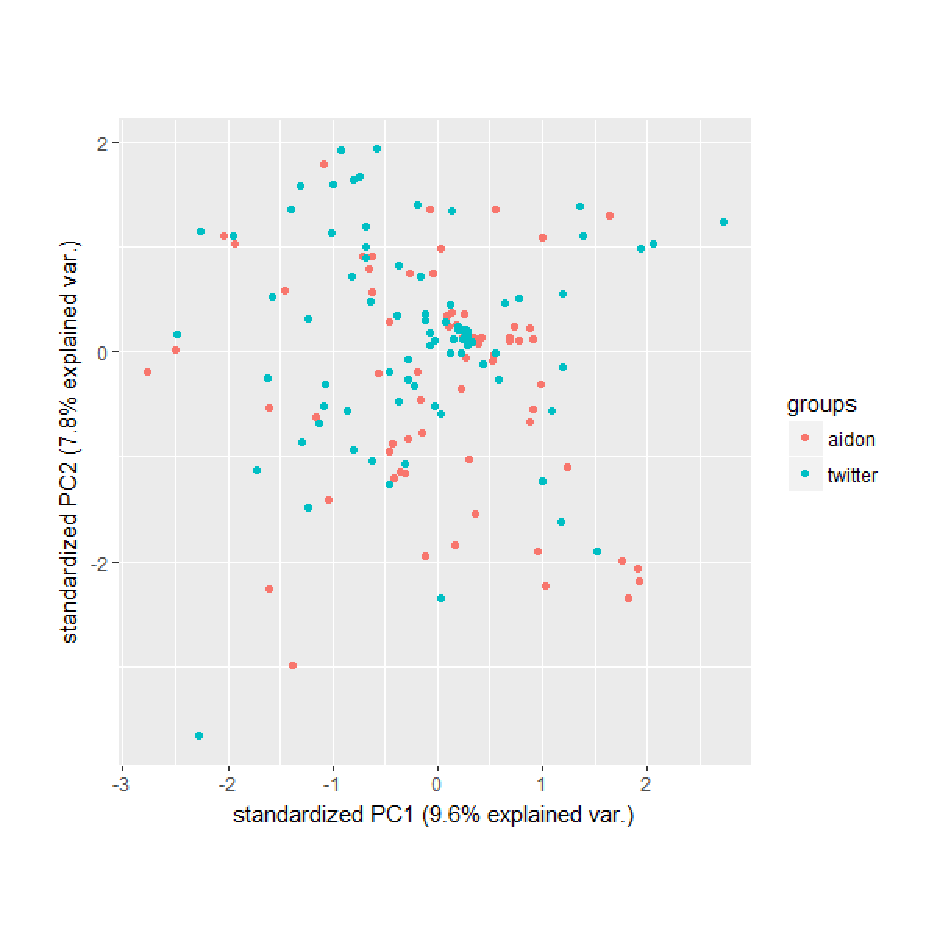
\includegraphics[width=13cm,clip]{aidon.pdf}
\caption{機械学習の相談ができるインスタンス}\label{aidon}
\end{figure}
\newpage

Twitterとスポーツバイクの話題が中心のインスタンスであるbicyclemstdn.jpの100のつぶやきをベクトル化し,主成分分析をした結果である.
\begin{figure}[h]
\centering
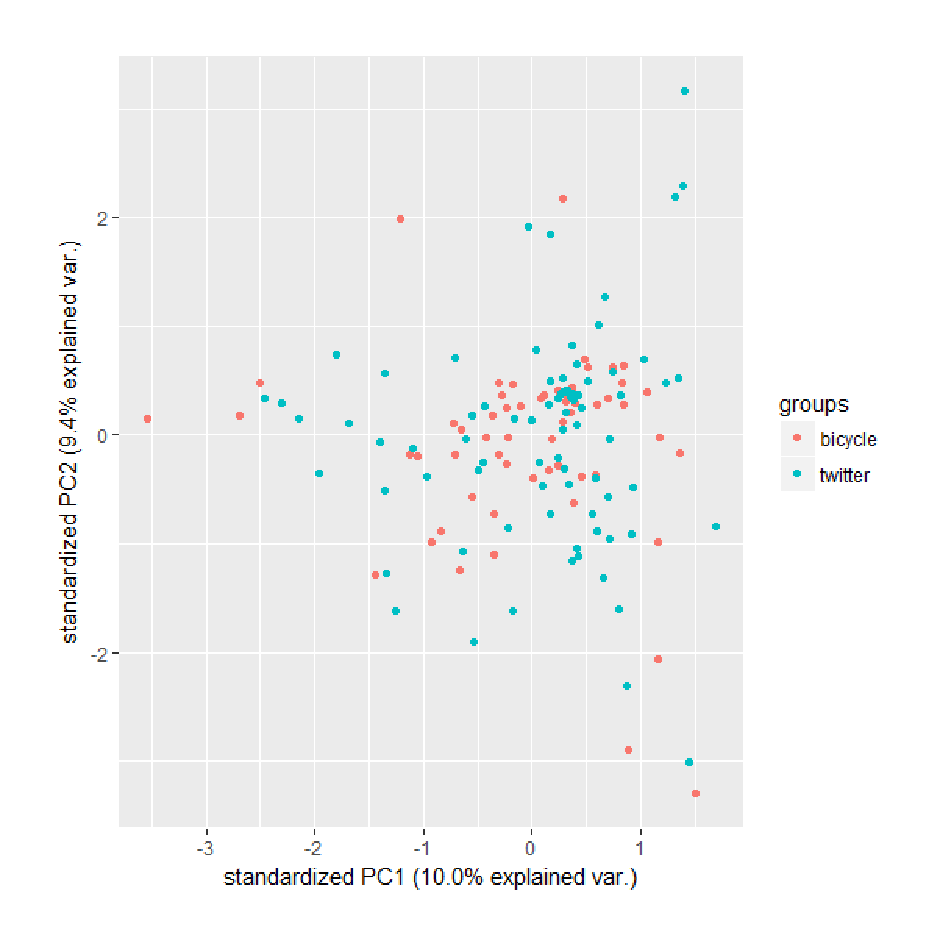
\includegraphics[width=13cm,clip]{bicycle.pdf}
\caption{スポーツバイクの話題が中心のインスタンス}\label{bicycle}
\end{figure}
\newpage

Twitterと猫好きのためのインスタンスであるcatdon.lifeの100のつぶやきをベクトル化し,主成分分析をした結果である.
\begin{figure}[h]
\centering
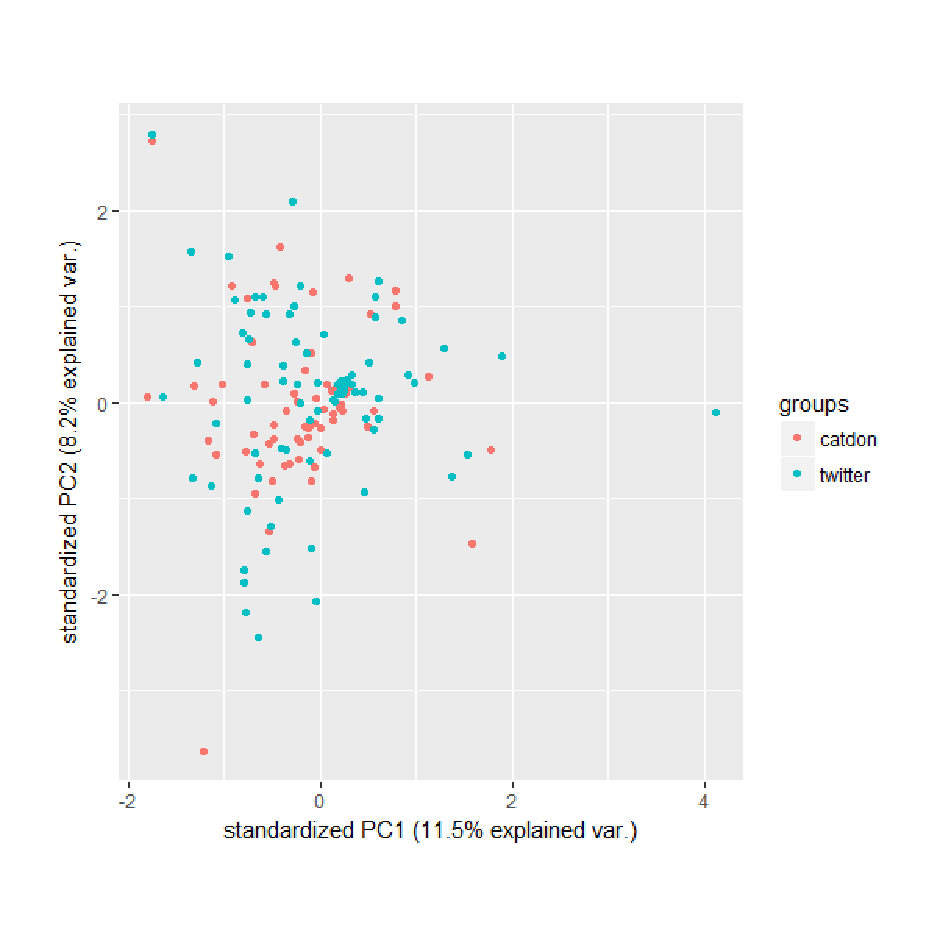
\includegraphics[width=13cm,clip]{catdon.pdf}
\caption{猫好きのためのインスタンス}\label{catdon}
\end{figure}
\newpage

Twitterとドラゴンクエスト10の話題が中心のインスタンスであるdq10.onlineの100のつぶやきをベクトル化し,主成分分析をした結果である.
\begin{figure}[h]
\centering
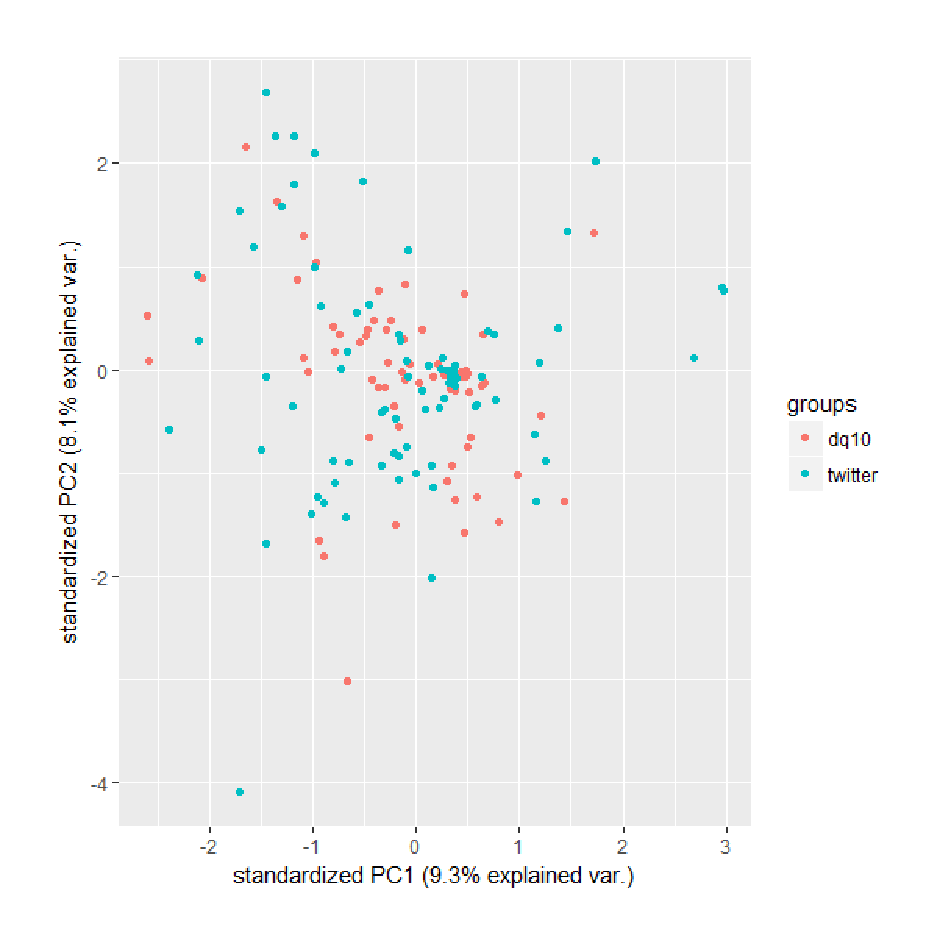
\includegraphics[width=13cm,clip]{dq10.pdf}
\caption{ドラゴンクエスト10の話題が中心のインスタンス}\label{dq10}
\end{figure}
\newpage

Twitterと映画好きのためのインスタンスであるeigadon.netの100のつぶやきをベクトル化し,主成分分析をした結果である.
\begin{figure}[h]
\centering
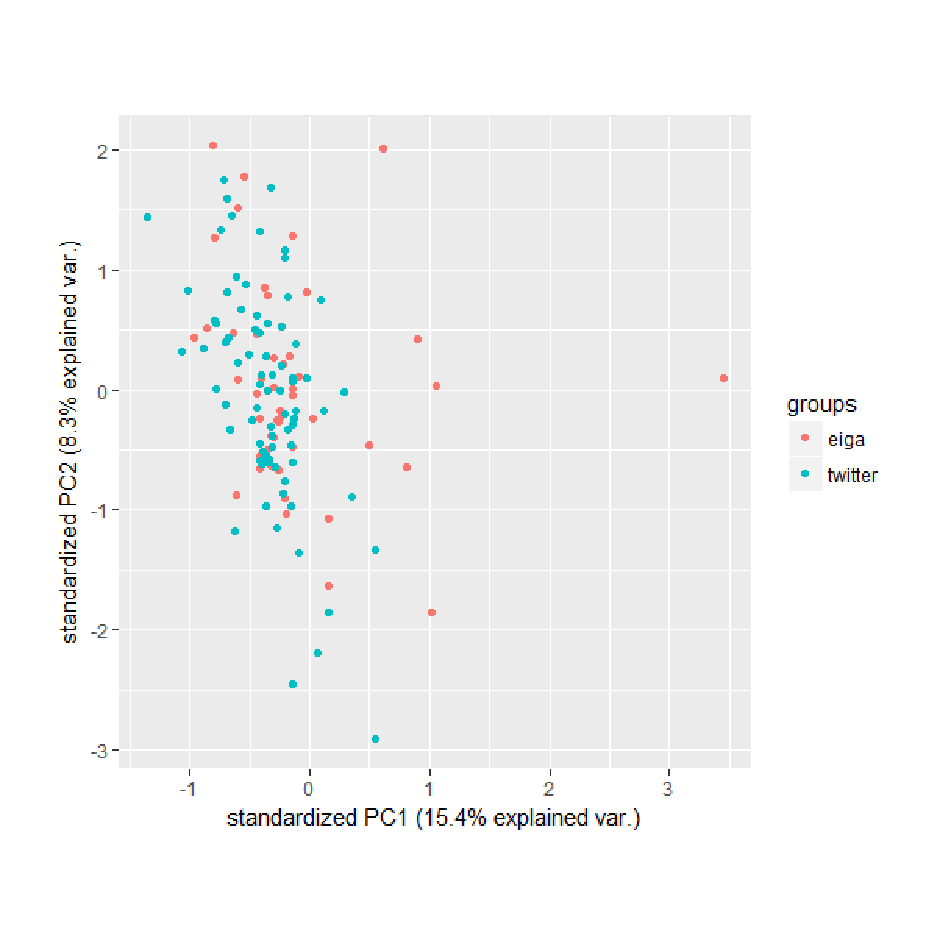
\includegraphics[width=13cm,clip]{eiga.pdf}
\caption{映画好きのためのインスタンス}\label{eiga}
\end{figure}
\newpage

Twitterと型月作品の話題が中心のインスタンスであるfgochiho.vipの100のつぶやきをベクトル化し,主成分分析をした結果である.
\begin{figure}[h]
\centering
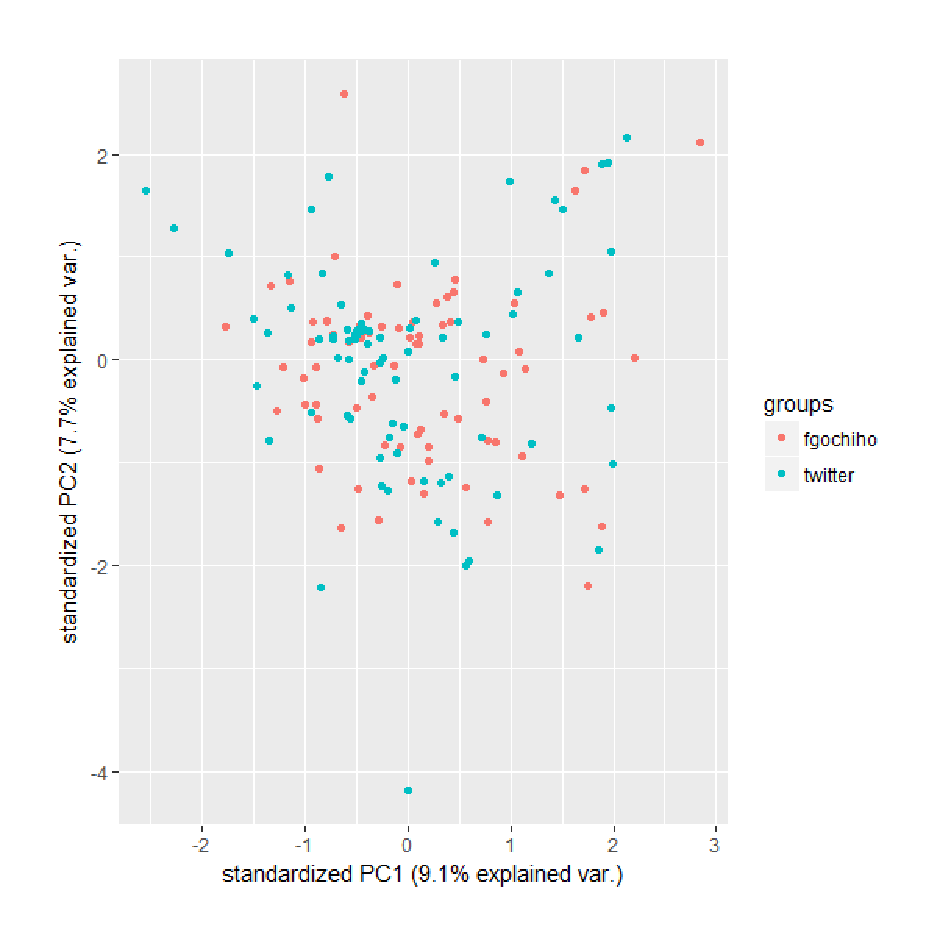
\includegraphics[width=13cm,clip]{fgochiho.pdf}
\caption{型月作品の話題が中心のインスタンス}\label{fgochiho}
\end{figure}
\newpage

Twitterとドワンゴが運営するインスタンスであるfriends.nicoの100のつぶやきをベクトル化し,主成分分析をした結果である.
\begin{figure}[h]
\centering
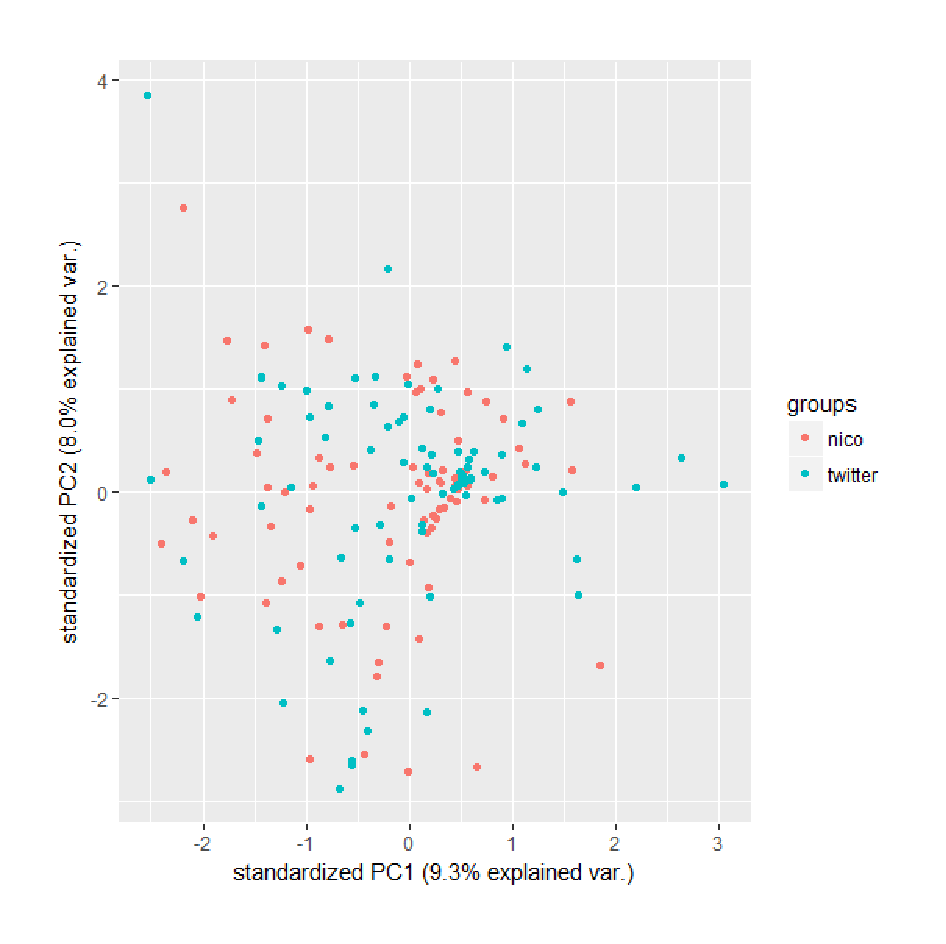
\includegraphics[width=13cm,clip]{nico.pdf}
\caption{ドワンゴが運営するインスタンス}\label{nico}
\end{figure}
\newpage

Twitterとゲーム制作者のインスタンスであるgamecreate.mstdn.cloudの100のつぶやきをベクトル化し,主成分分析をした結果である.
\begin{figure}[h]
\centering
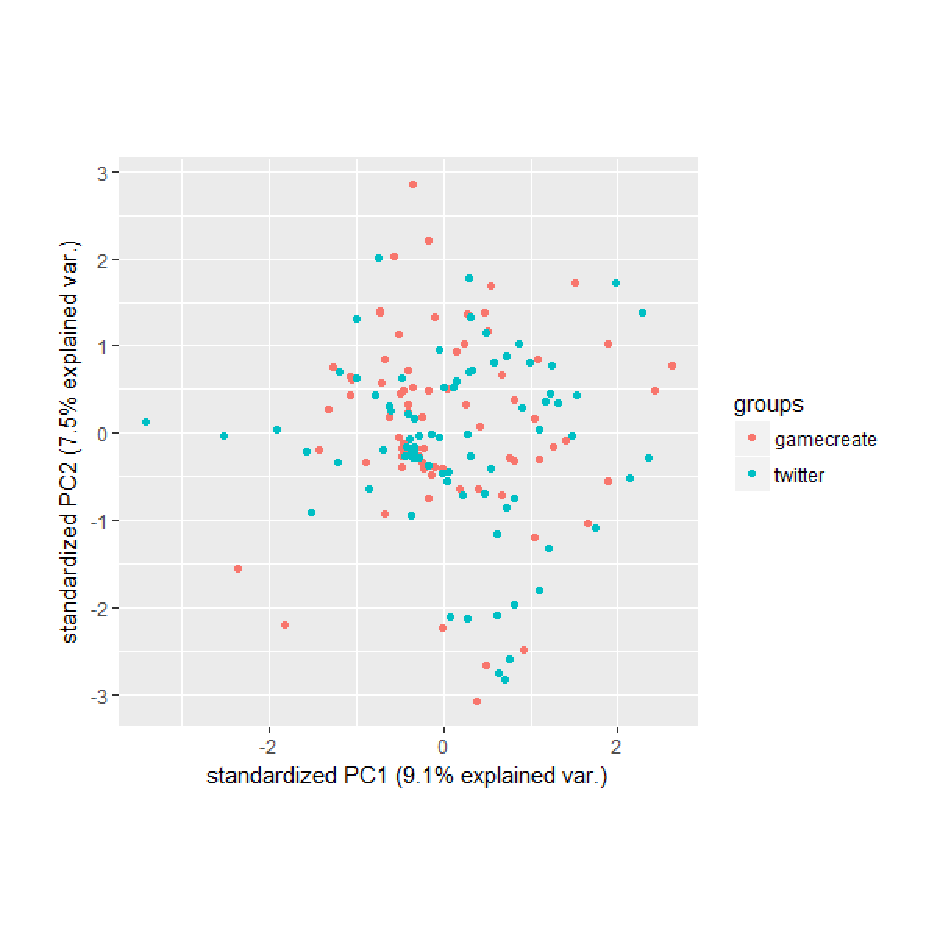
\includegraphics[width=13cm,clip]{gamecreate.pdf}
\caption{ゲーム制作者のインスタンス}\label{gamecreate}
\end{figure}
\newpage

TwitterとSplatoonの話題が中心のインスタンスであるika.queloud.netの100のつぶやきをベクトル化し,主成分分析した結果である.
\begin{figure}[h]
\centering
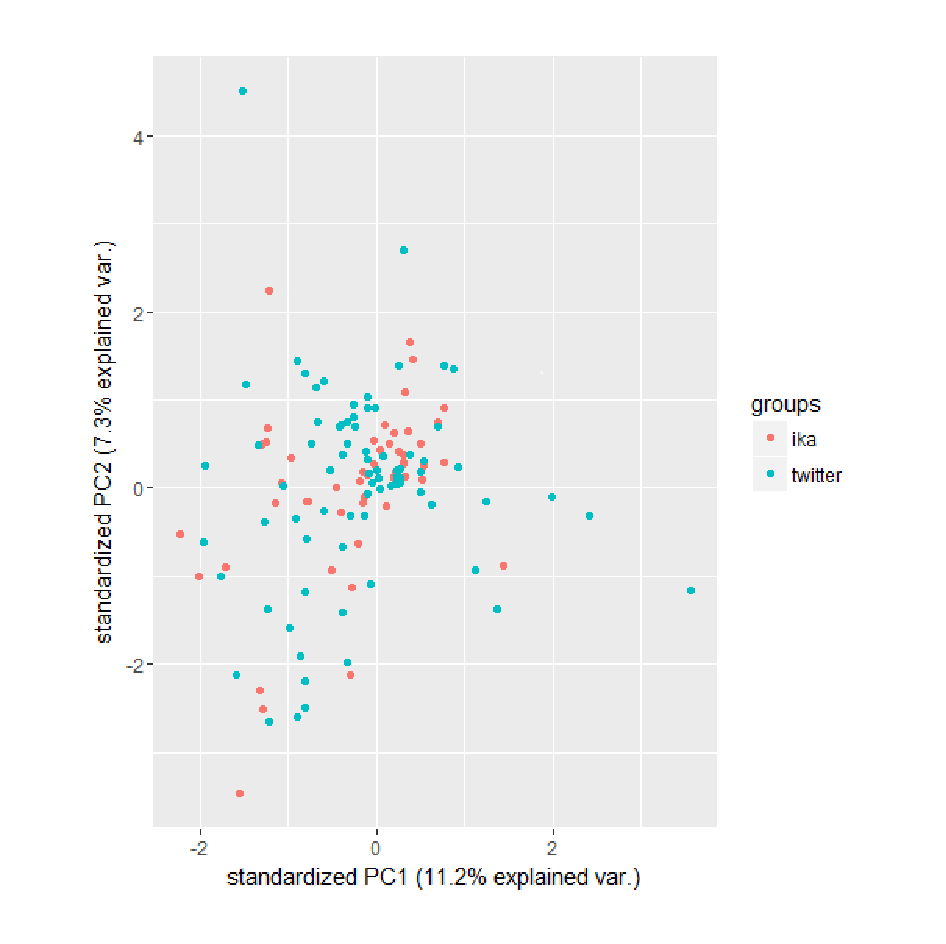
\includegraphics[width=13cm,clip]{ika.pdf}
\caption{Splatoonの話題が中心のインスタンス}\label{ika}
\end{figure}
\newpage

Twitterとアイドルマスターの話題が中心のインスタンスであるimastodon.netの100のつぶやきをベクトル化し,主成分分析した結果である.
\begin{figure}[h]
\centering
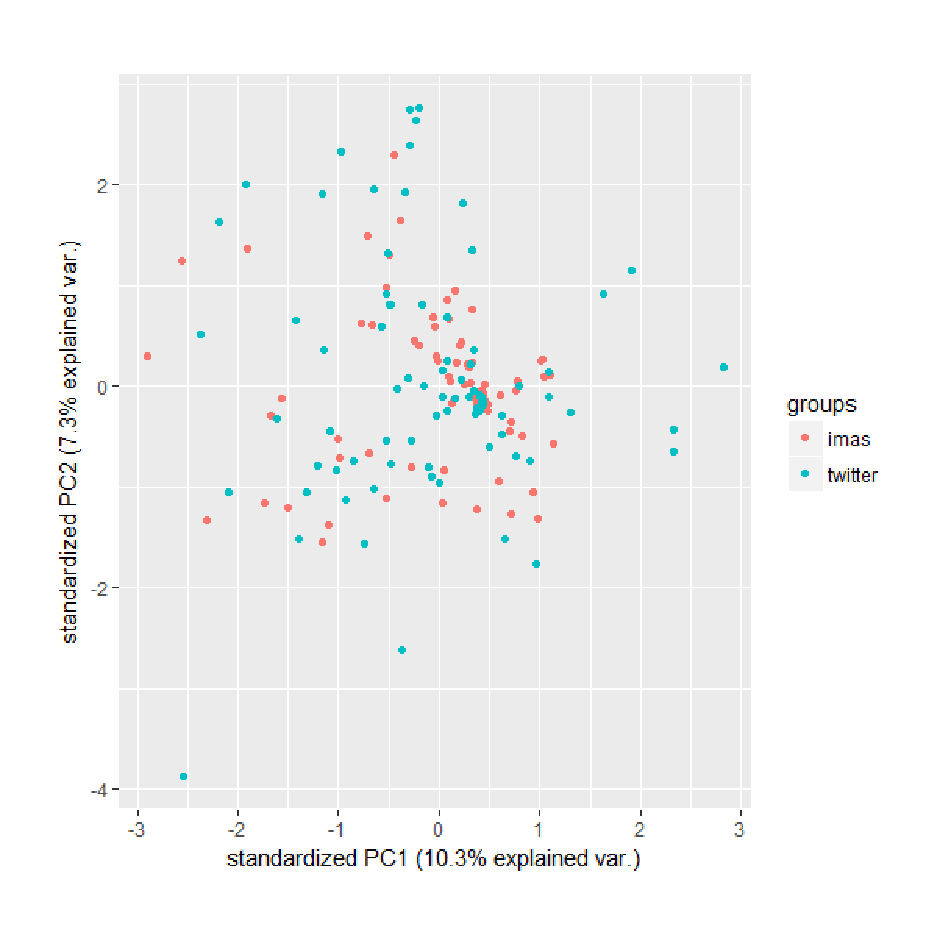
\includegraphics[width=13cm,clip]{imas.pdf}
\caption{アイドルマスターの話題が中心のインスタンス}\label{imas}
\end{figure}
\newpage

Twitterとカードキャプターさくら/CLAMPの話題が中心のインスタンスであるkero.ccsakura.jpの100のつぶやきをベクトル化し,主成分分析した結果である.
\begin{figure}[h]
\centering
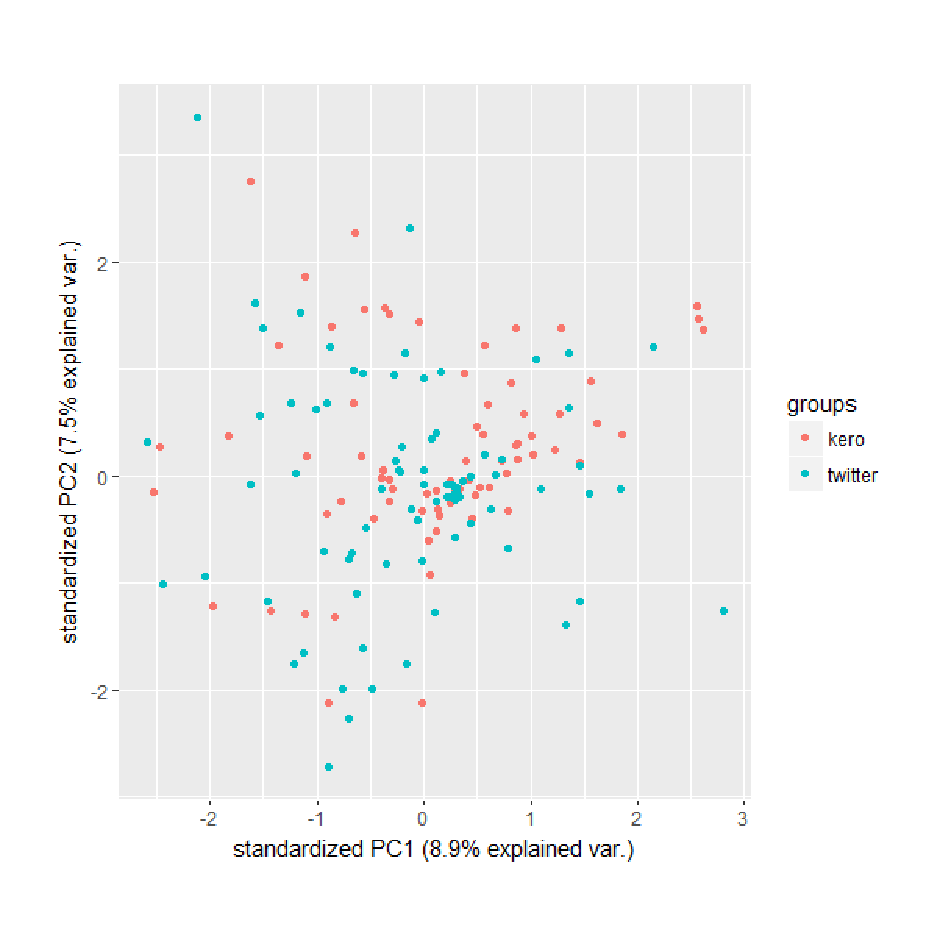
\includegraphics[width=13cm,clip]{kero.pdf}
\caption{カードキャプターさくら/CLAMPの話題が中心のインスタンス}\label{kero}
\end{figure}
\newpage

Twitterとアイカツ!の話題が中心のインスタンスであるkirakiratter.comの100のつぶやきをベクトル化し,主成分分析した結果である.
\begin{figure}[h]
\centering
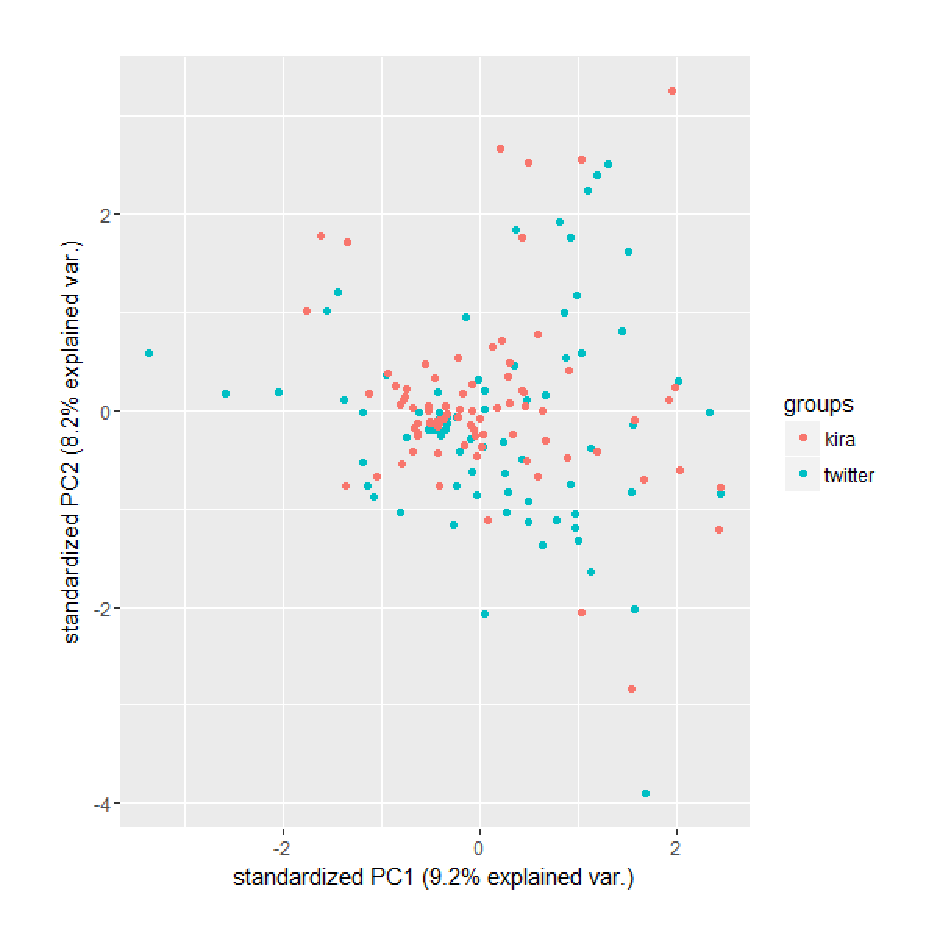
\includegraphics[width=13cm,clip]{kira.pdf}
\caption{アイカツ!の話題が中心のインスタンス}\label{kira}
\end{figure}
\newpage

Twitterと婚活している人が集うインスタンスであるkonkat.jpの100のつぶやきをベクトル化し,主成分分析した結果である.
\begin{figure}[h]
\centering
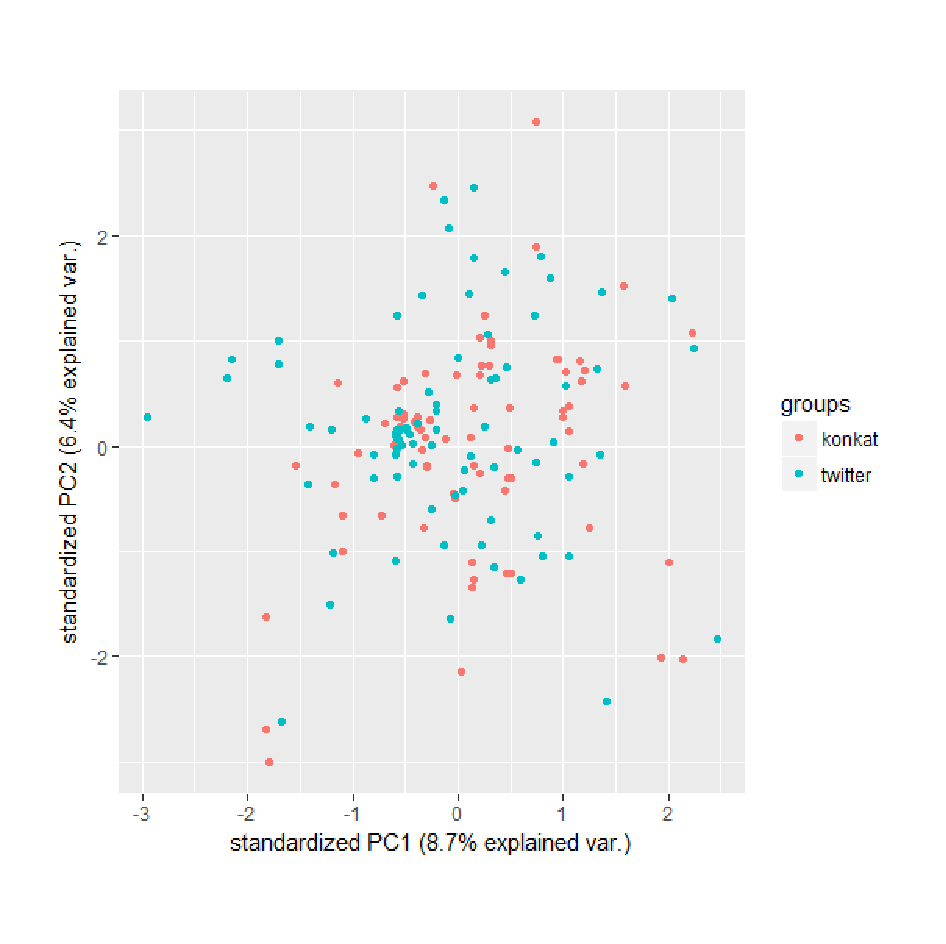
\includegraphics[width=13cm,clip]{konkat.pdf}
\caption{婚活している人が集うインスタンス}\label{konkat}
\end{figure}
\newpage

Twitterとクラゲ専門のインスタンスであるkurage.ccの100のつぶやきをベクトル化し,主成分分析した結果である.
\begin{figure}[h]
\centering
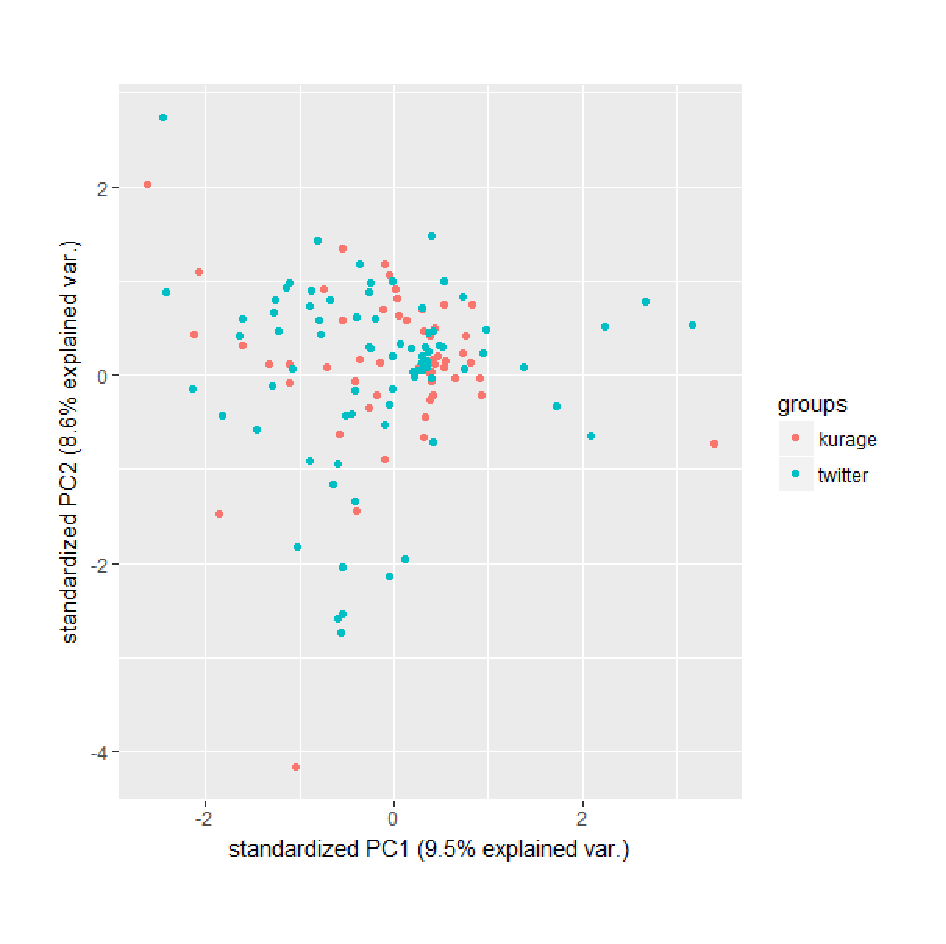
\includegraphics[width=13cm,clip]{kurage.pdf}
\caption{クラゲ専門のインスタンス}\label{kurage}
\end{figure}
\newpage

Twitterとアニメ,ゲームの話題が中心のインスタンスであるmast.moeの100のつぶやきをベクトル化し,主成分分析した結果である.
\begin{figure}[h]
\centering
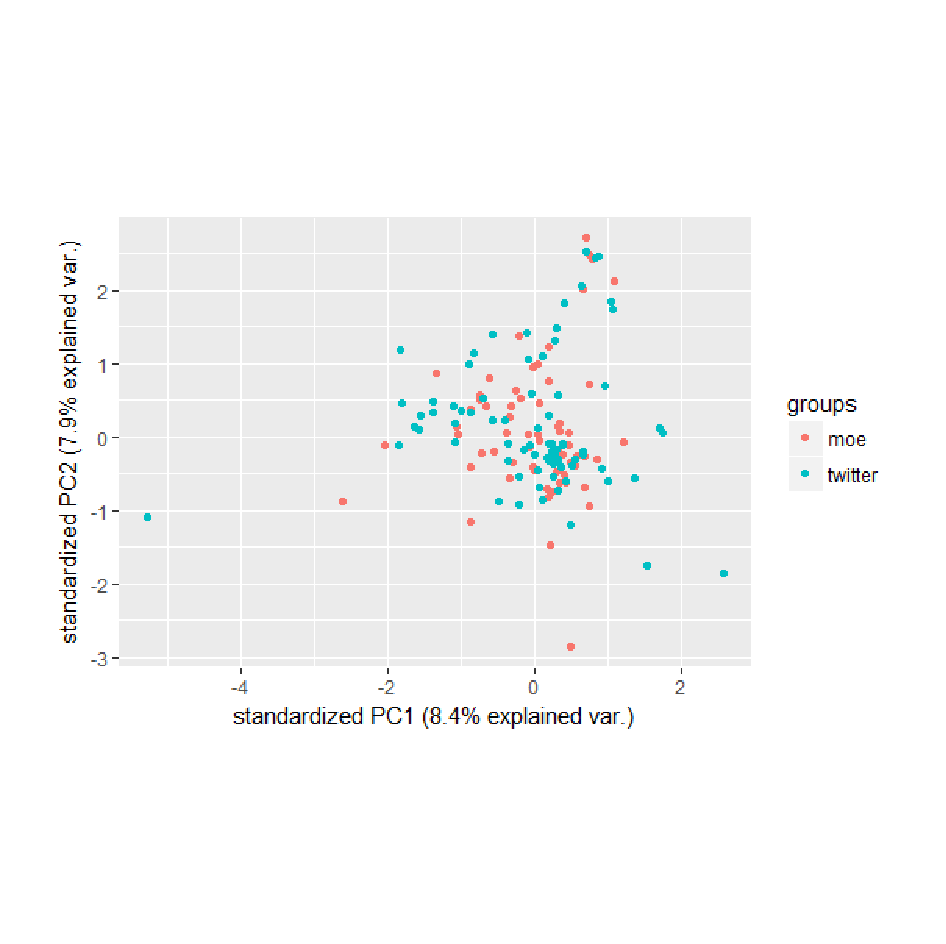
\includegraphics[width=13cm,clip]{moe.pdf}
\caption{アニメ,ゲームの話題が中心のインスタンス}\label{moe}
\end{figure}
\newpage

Twitterと仮想通貨ユーザーのためのインスタンスであるmastodon.bitbank.ccの100のつぶやきをベクトル化し,主成分分析した結果である.
\begin{figure}[h]
\centering
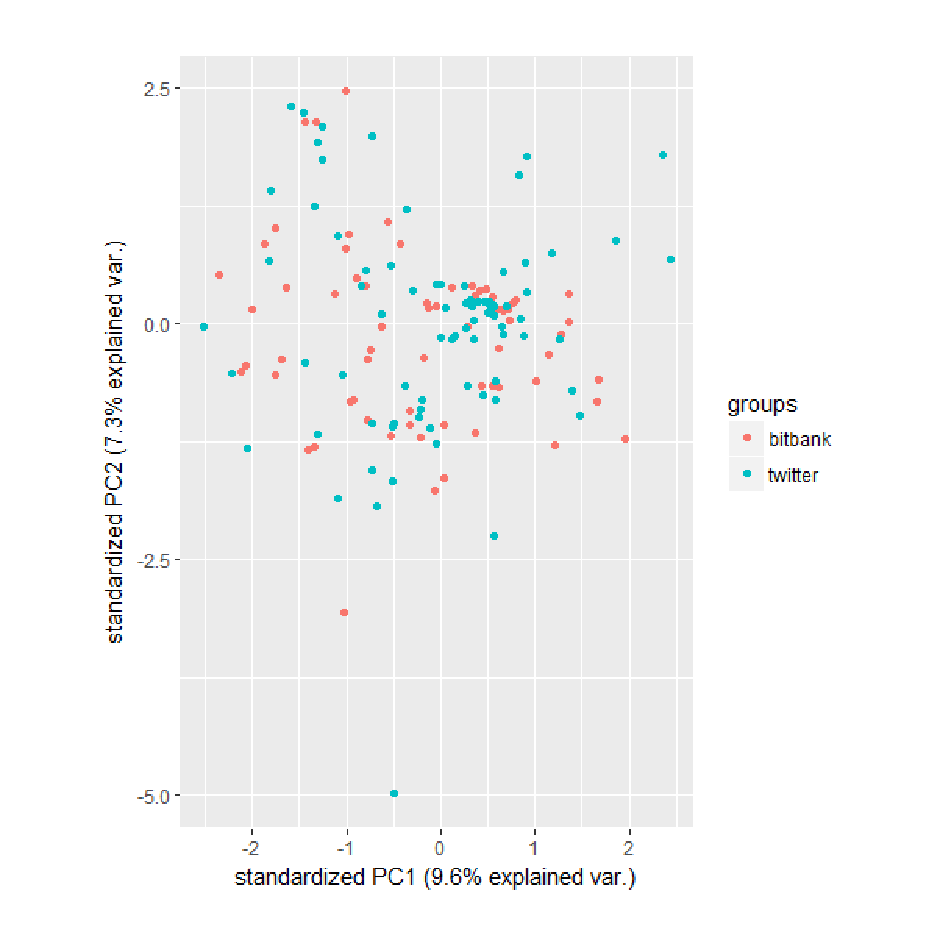
\includegraphics[width=13cm,clip]{bitbank.pdf}
\caption{仮想通貨ユーザーのためのインスタンス}\label{bitbank}
\end{figure}
\newpage

Twitterと宇宙開発と天文観測の話題が中心のインスタンスであるmastodon.cosmicanimal.jpの100のつぶやきをベクトル化し,主成分分析した結果である.
\begin{figure}[h]
\centering
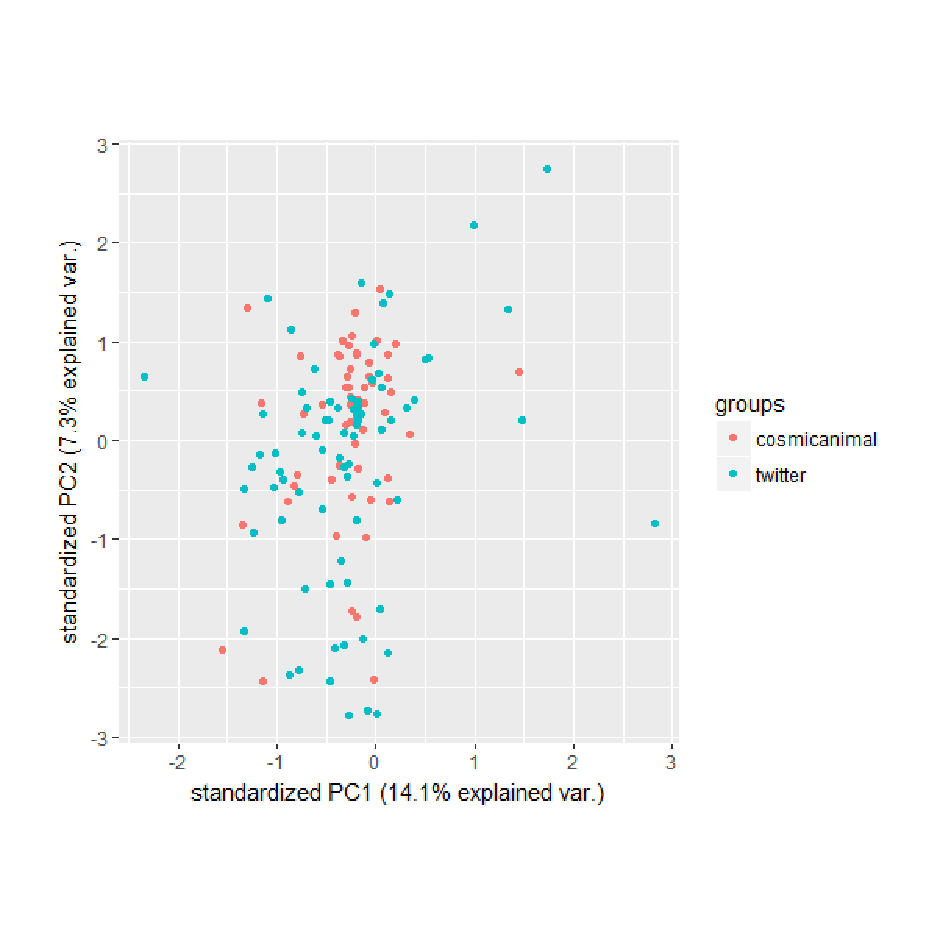
\includegraphics[width=13cm,clip]{cosmicanimal.pdf}
\caption{宇宙開発と天文観測の話題が中心のインスタンス}\label{cosmicanimal}
\end{figure}
\newpage

Twitterと釣り人専用のインスタンスであるmastodon.fishingの100のつぶやきをベクトル化し,主成分分析した結果である.
\begin{figure}[h]
\centering
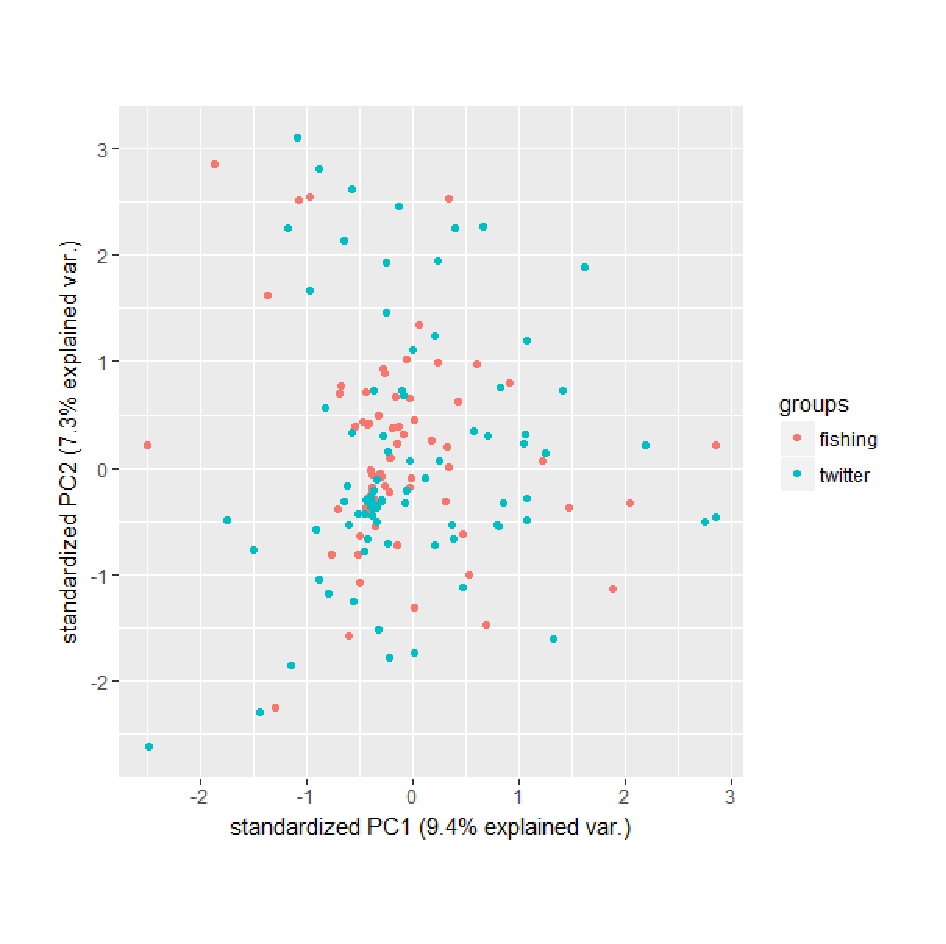
\includegraphics[width=13cm,clip]{fishing.pdf}
\caption{釣り人専用のインスタンス}\label{fishing}
\end{figure}
\newpage

Twitterと横浜の話題が中心のインスタンスであるmastodon.yokohamaの100のつぶやきをベクトル化し,主成分分析した結果である.
\begin{figure}[h]
\centering
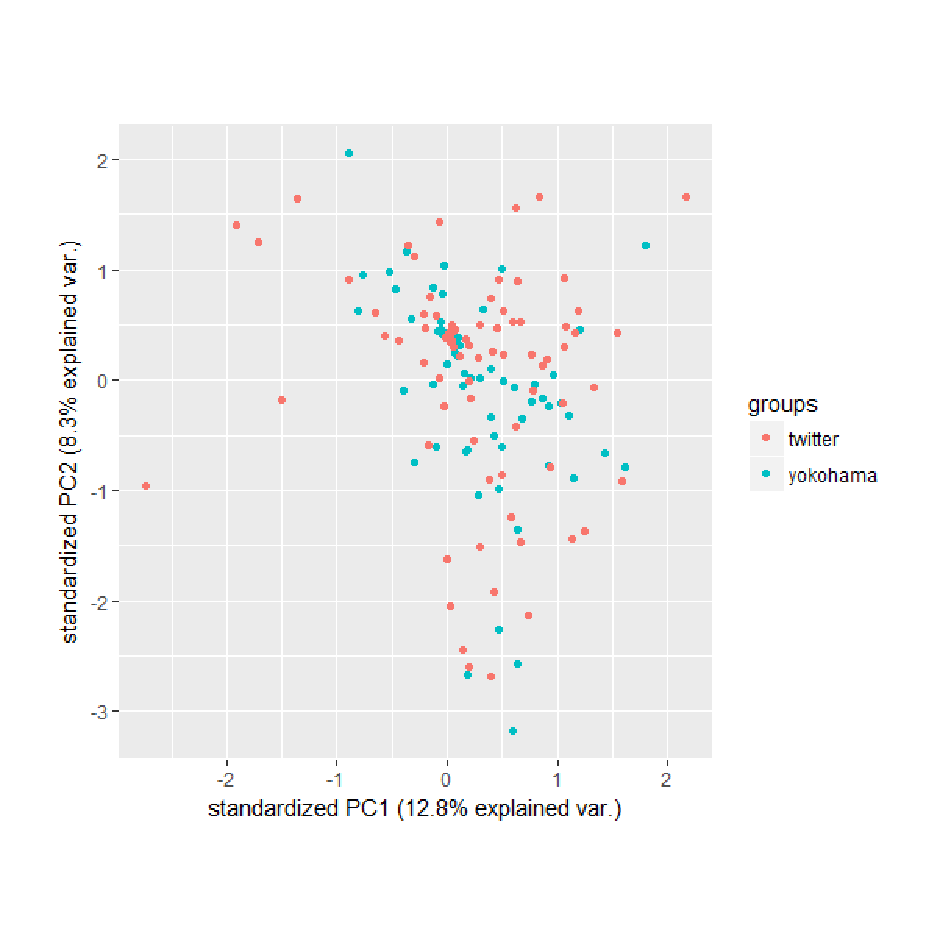
\includegraphics[width=13cm,clip]{yokohama.pdf}
\caption{横浜の話題が中心のインスタンス}\label{yokohama}
\end{figure}
\newpage

Twitterと北海道の話題が中心のインスタンスであるmstdn.hokkaido.jpの100のつぶやきをベクトル化し,主成分分析した結果である.
\begin{figure}[h]
\centering
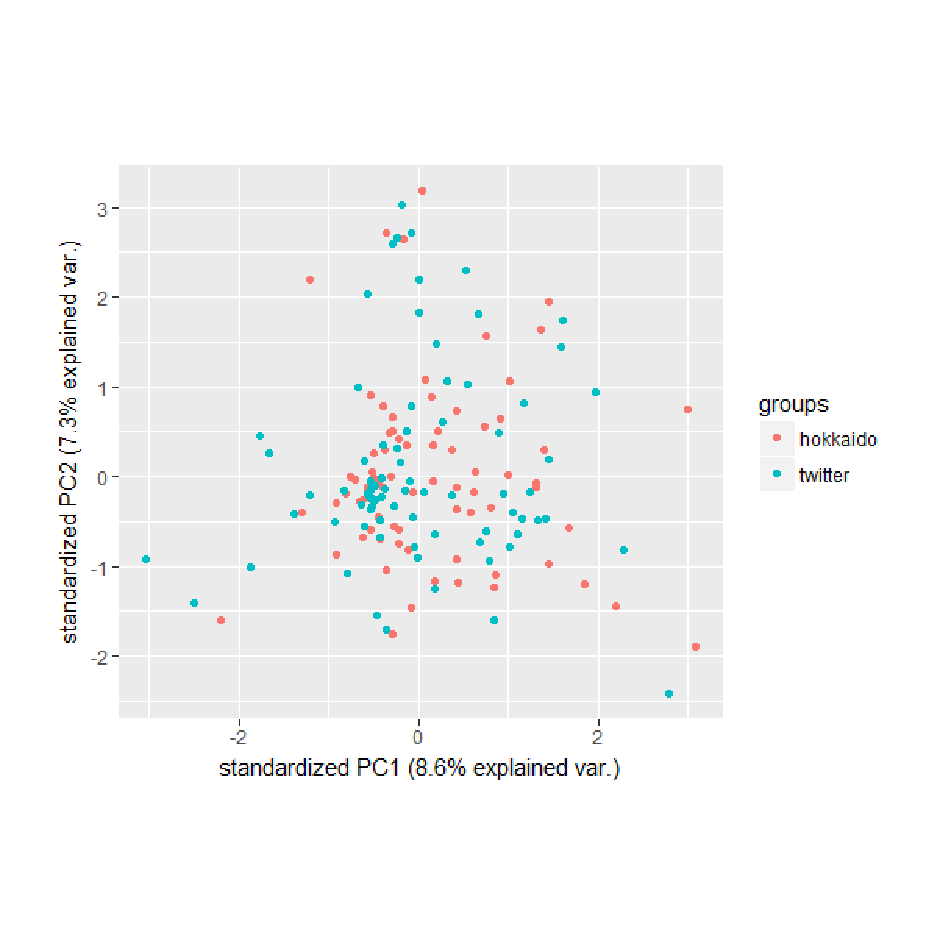
\includegraphics[width=13cm,clip]{hokkaido.pdf}
\caption{北海道の話題が中心のインスタンス}\label{hokkaido}
\end{figure}
\newpage

Twitterと話題が自由なインスタンスであるmstdn.jpの100のつぶやきをベクトル化し,主成分分析をした結果である.
\begin{figure}[h]
\centering
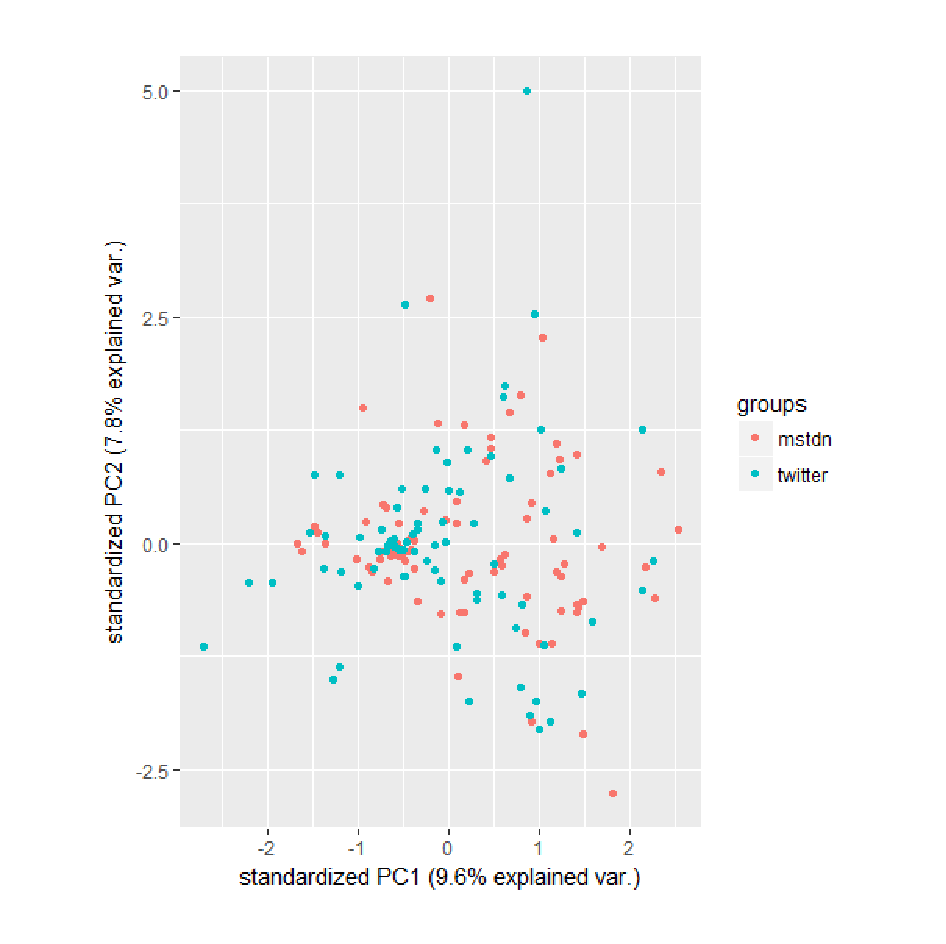
\includegraphics[width=13cm,clip]{mstdn.pdf}
\caption{話題が自由なインスタンス}\label{mstdn}
\end{figure}
\newpage

Twitterと大阪の話題が中心のインスタンスであるmstdn.osakaの100のつぶやきをベクトル化し,主成分分析をした結果である.
\begin{figure}[h]
\centering
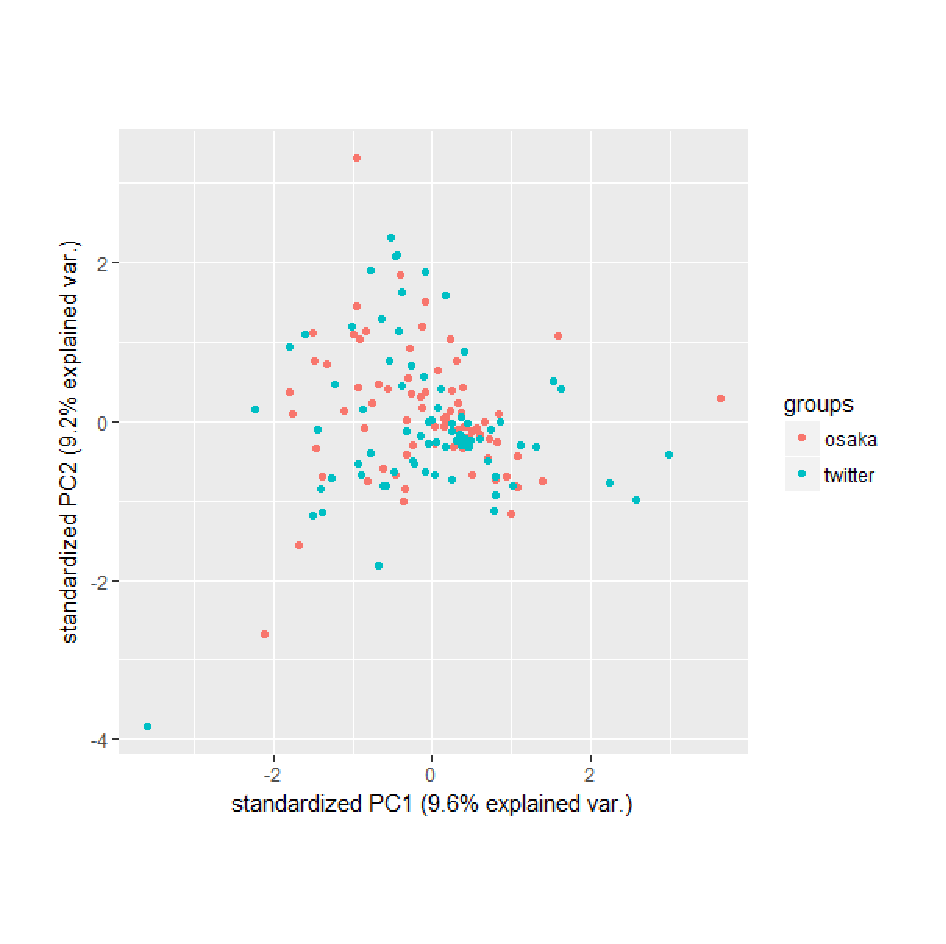
\includegraphics[width=13cm,clip]{osaka.pdf}
\caption{大阪の話題が中心のインスタンス}\label{osaka}
\end{figure}
\newpage

Twitterとサッカーの話題が中心のインスタンスであるmstdn-football.jpの100のつぶやきをベクトル化し,主成分分析をした結果である.
\begin{figure}[h]
\centering
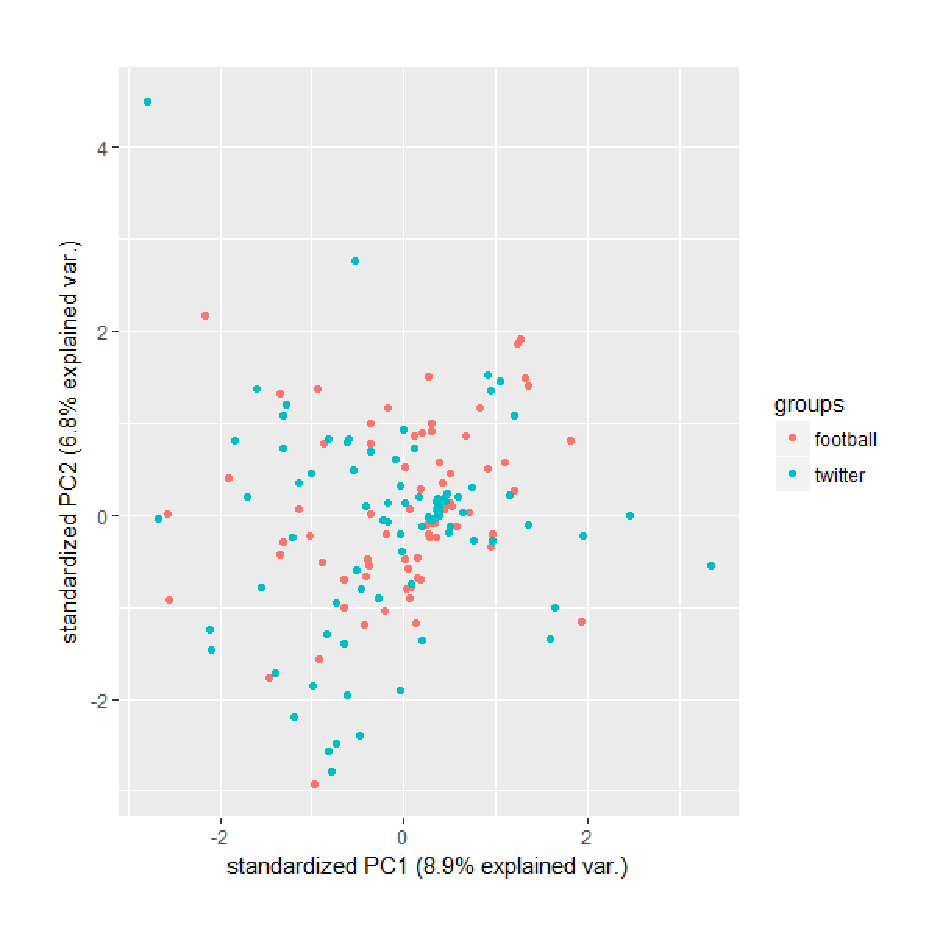
\includegraphics[width=13cm,clip]{football.pdf}
\caption{サッカーの話題が中心のインスタンス}\label{football}
\end{figure}
\newpage

Twitterと金沢市の話題が中心のインスタンスであるmstdn-kanazawa.jpの100のつぶやきをベクトル化し,主成分分析をした結果である.
\begin{figure}[h]
\centering
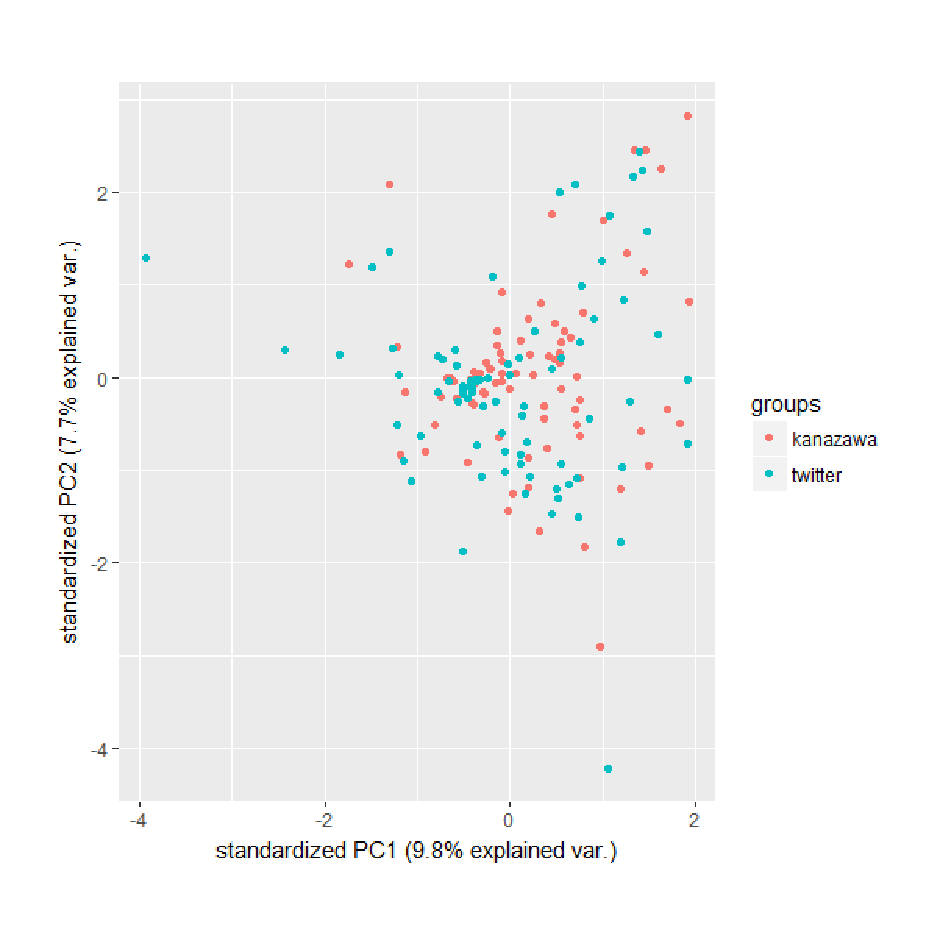
\includegraphics[width=13cm,clip]{kanazawa.pdf}
\caption{金沢市の話題が中心のインスタンス}\label{kanazawa}
\end{figure}
\newpage

Twitterときぼうソフトが運営する、初めてFacebookログインとBBCodeによる文字の回転に対応したインスタンスであるnow.kibousoft.co.jpの100のつぶやきをベクトル化し,主成分分析をした結果である.
\begin{figure}[h]
\centering
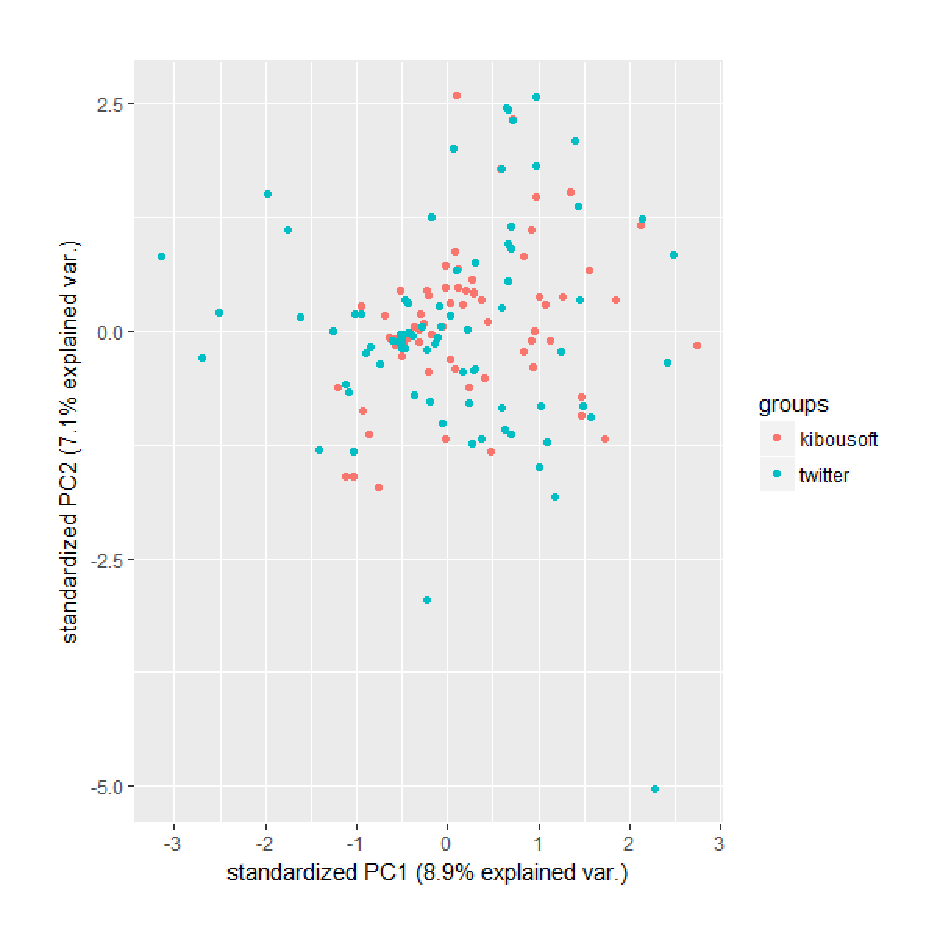
\includegraphics[width=13cm,clip]{kibousoft.pdf}
\caption{きぼうソフトが運営するインスタンス}\label{kibousoft}
\end{figure}
\newpage

Twitterとピクシブが運営するインスタンスであるpawoo.netの100のつぶやきをベクトル化し,主成分分析をした結果である.
\begin{figure}[h]
\centering
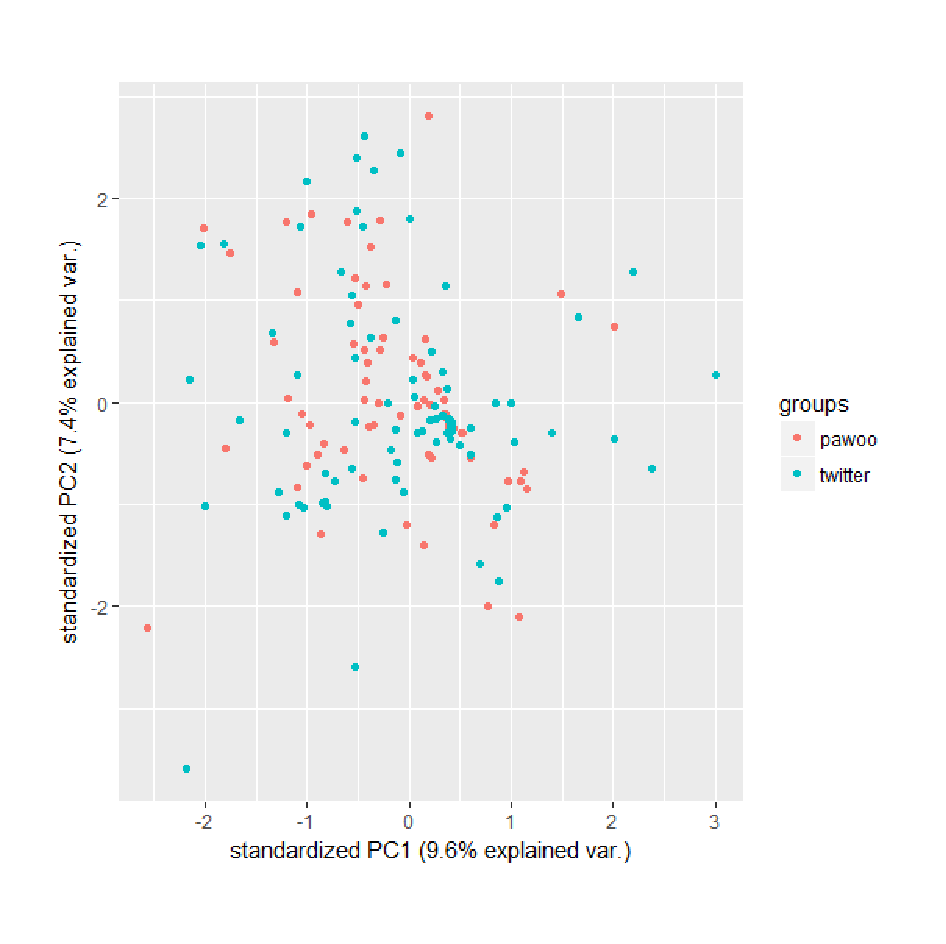
\includegraphics[width=13cm,clip]{pawoo.pdf}
\caption{ピクシブが運営するインスタンス}\label{pawoo}
\end{figure}
\newpage

Twitterとラグナロクオンラインの話題が中心のインスタンスであるro-mastodon.puyo.jpの100のつぶやきをベクトル化し,主成分分析をした結果である.
\begin{figure}[h]
\centering
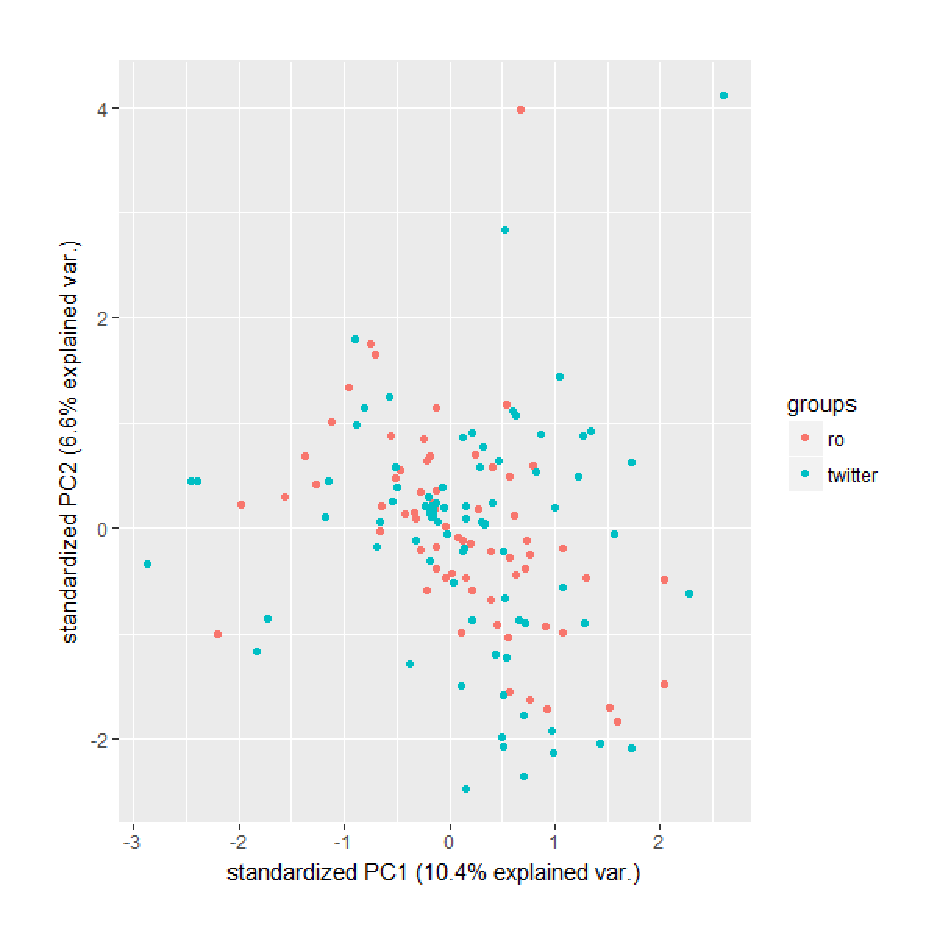
\includegraphics[width=13cm,clip]{ro.pdf}
\caption{ラグナロクオンラインの話題が中心のインスタンス}\label{ro}
\end{figure}
\newpage

Twitterとオープンソースのプロジェクト管理ツール「Redmine」の話題が中心のインスタンスであるro-mastodon.puyo.jpの100のつぶやきをベクトル化し,主成分分析をした結果である.
\begin{figure}[h]
\centering
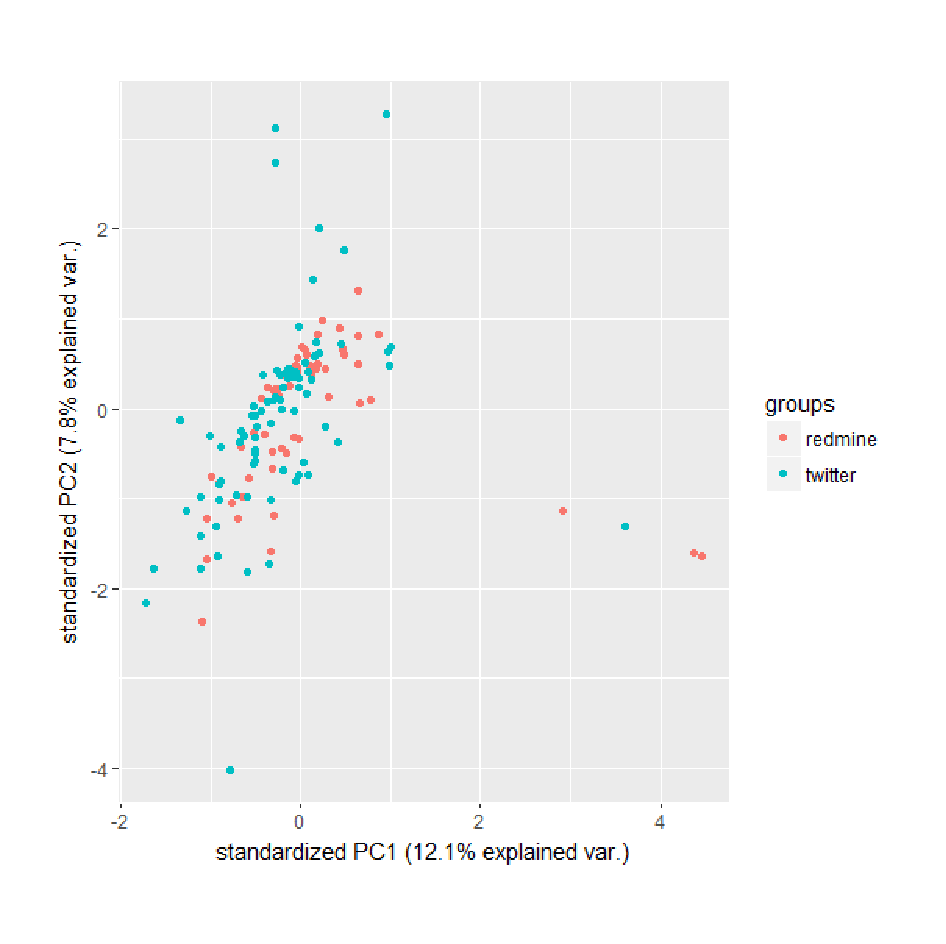
\includegraphics[width=13cm,clip]{redmine.pdf}
\caption{オープンソースのプロジェクト管理ツール「Redmine」の話題が中心のインスタンス}\label{redmine}
\end{figure}
\newpage

Twitterとニッポン放送が運営するインスタンスであるtuner.1242.comの100のつぶやきをベクトル化し,主成分分析をした結果である.
\begin{figure}[h]
\centering
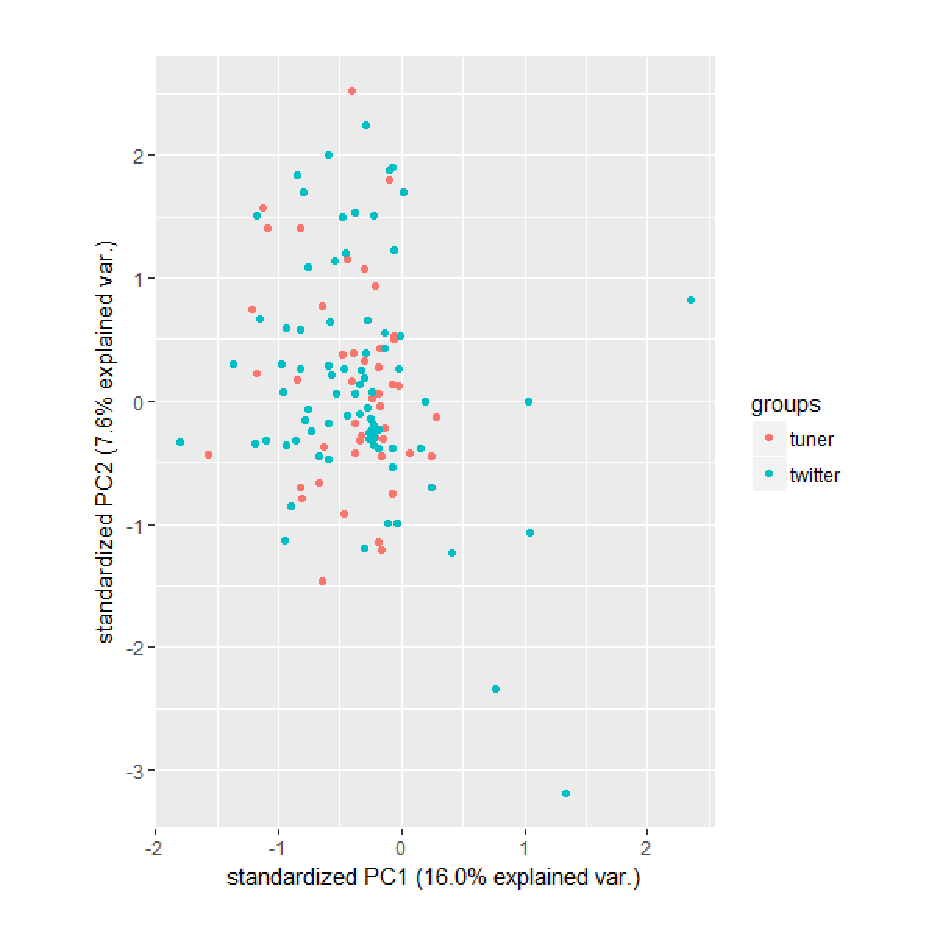
\includegraphics[width=13cm,clip]{tuner.pdf}
\caption{ニッポン放送が運営するインスタンス}\label{tuner}
\end{figure}
\newpage

Twitterとボカロクラスタが集うインスタンスであるvocalodon.netの100のつぶやきをベクトル化し,主成分分析をした結果である.
\begin{figure}[h]
\centering
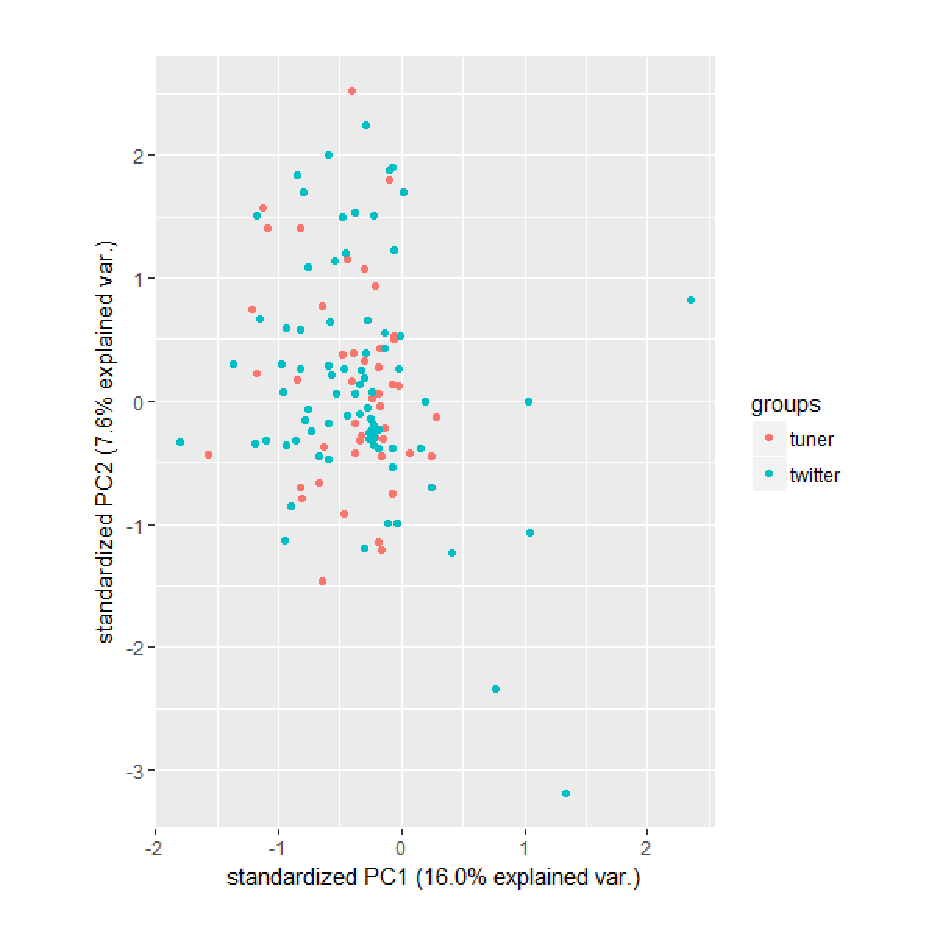
\includegraphics[width=13cm,clip]{tuner.pdf}
\caption{ボカロクラスタが集うインスタンス}\label{tuner}
\end{figure}
\newpage

\chapter{考察}
主成分分析の結果を可視化したバイプロットでは,話題が幅広いTwitterのつぶやきは拡散し,話題が限定されているMastodonのつぶやきは局所化することが予想されたのだが,分析結果は図のように,両者に明確な違いは見られなかった.このことは,Word2vecと主成分分析という方法では,人間が簡単に理解しているような,話題の違いを検出できないことを示唆している.
\chapter{結論}
本研究で用いたWord2vecと主成分分析という手法で話題の広さの違いを識別することは困難だということが分かった.つぶやき単体ではなく,大量のつぶやきをまとめてベクトル化する手法を試みることが今後の課題であろう.
\bibliographystyle{junsrt}
\bibliography{biblio}%「biblio.bib」というファイルが必要.
\chapter*{謝辞}\addcontentsline{toc}{chapter}{謝辞}

本論文を作成するにあたり,ご指導を頂いた卒業論文指導教員の矢吹太朗准教授に感謝致します.先生にはお話を通じて社会を見る視野を広げていただきました.そして多くのご指摘やご助言を下さいました矢吹研究室の皆様に心から感謝します.


\end{document}
\end{lstlisting}